\documentclass[ngerman]{latex-classes/summary}

\title{Zusammenfassung Datenbanksysteme}
\author{Jens Ochsenmeier}

% ENV -- FRAGEN
\newenvironment{fragen}
  {
    \begin{tcolorbox}[colback=black!5!white,colframe=white!75!black,title=Prüfungsfragen,arc=0mm]
      \begin{enumerate}
      \setlength\itemsep{0em}
  }
  {
      \end{enumerate}
    \end{tcolorbox}
  }

\begin{document}

  \section{Einleitung}
\label{sec:einleitung}

\paragraph{Motivation}
\begin{itemize}
  \item 50\% weniger Aufwand bei Anwendungsentwicklung mit DB
  \item Ermöglicht neue Anwendungen, die ohne DB zu komplex wären
  \item Ausfaktorisieren der Verwaltung großer Datenmengen
  \item \textbf{ohne Datenbanken}:
  \begin{itemize}
    \item Daten in Dateien abgelegt, Zugriffsfunktionalität Teil der Anwendung
    \item Redundanz (in Daten und Funktionalität)
    \item Programme oft nicht \emph{atomar} (= Programm wird entweder ganz oder gar nicht ausgeführt) --- nur bei nicht fehlerfreien Systemen relevant
    \item \emph{Transaktionen} (= Programm oder Kommandofolge) oft nicht \emph{isoliert} (= keine inkonsistenten Zwischenzustände sichtbar) --- nur bei mehreren Transaktionen, aber auch bei fehlerfreien Systemen relevant
    \item Nebenläufigkeit (\emph{concurrency} --- paralleler Zugriff auf dieselben Daten) schwer umsetzbar
    \item Anwendungsentwicklung abhängig von der physischen Repräsentation der Daten (z.B. Datenspeicherung als Tabelle: Reihenfolge Zeilen/Spalten muss bekannt sein)
    \item Datenschutz (kein unbefugter Zugriff) nicht gewährleistet
    \item Datensicherheit (kein Datenverlust, insb. bei Defekten) nicht gewährleistet
  \end{itemize}
\end{itemize}

\paragraph{Relationale Datenbanken}
\begin{itemize}
  \item auch \textbf{RDBMS} (\emph{relational database management system})
  \item[\( \cong \)] Menge von Tabellen
  \item Relation = Menge von Tupeln = Tabelle
\end{itemize}

\paragraph{RDBMS --- Terminologie}
\begin{itemize}
  \item \textbf{Relationenschema}: \emph{Fett} geschrieben
  \item \textbf{Relation}: Weitere Einträge der Tabelle
  \item \textbf{Tupel}: Eine Zeile der Tabelle
  \item \textbf{Attribut}: Spaltenüberschrift
  \item \textbf{Relationenname}: Name der Tabelle
  \item \textbf{DBS}: Datenbanksystem = DBMS + Datenbank(en)
  \item \textbf{Schlüssel}: Attribut, das nicht doppelt vergeben werden darf
  \item \textbf{Fremdschlüssel}: Attr taucht in anderem Relationenschema als Schlüssel auf
  \item \textbf{Integritätsbedingungen}:
  \begin{itemize}
    \item \emph{lokal}: Schlüssel in Relationenschema
    \item \emph{global}: Fremdschlüssel in Datenbankschema
  \end{itemize}
  \item \textbf{DB-Schema}: = Menge Relationsschemata + globale Integritätsbedingungen
  \item \textbf{Sicht} (\emph{view}): Häufig vorkommende Datenabfrage, kann mit Sichtnamen als "`virtuelle"' Tabelle gespeichert werden \\*
  \begin{lstlisting}[language=sql]
    create view CArtist as
      select NAME, JAHR
      from Kuenstler
      where LAND == "Kanada"
  \end{lstlisting}
  \item Verwendung wie "`normale"' Relation:
  \begin{lstlisting}[language=sql]
    select * from CArtist where JAHR < 2000
  \end{lstlisting}
  \item Nutzung für Datenschutz: Unterschiedliche Benutzer sehen unterschiedlichen DB-Ausschnitt
\end{itemize}

\paragraph{RDBMS --- Anfrageoperationen}
\begin{itemize}
  \item \textbf{Selektion}: Zeilen (Tupel) wählen (\( \sigma_{\text{KID}=1012}(\text{Titel}) \))
  \item \textbf{Projektion}: Spalten (Attribute) wählen (\( \pi_{\text{KID, NAME}}(\text{Kuenstler}) \))
  \item Beispiel komplexer Ausdruck: \( \pi_{\text{NAME}, \text{ART}}(\sigma_{\text{KID}=1012}(\text{Titel})) \)
  \begin{figure}[H]\centering\label{SelektionProjektion}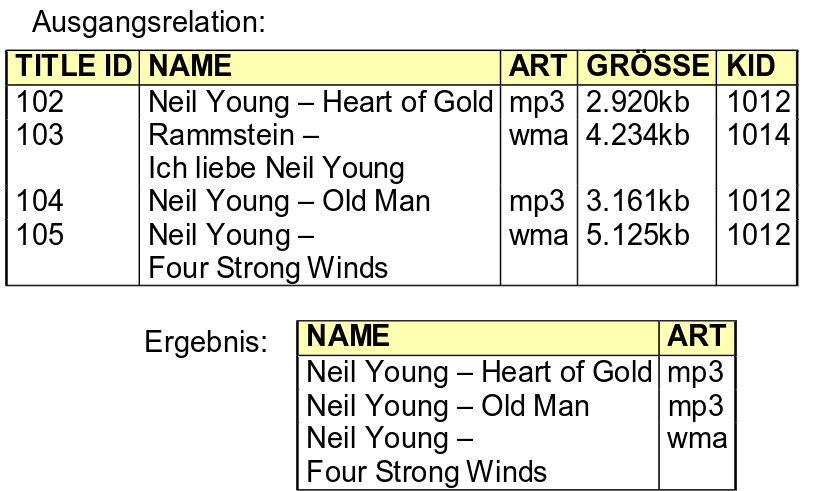
\includegraphics[width=0.3\textwidth]{SelektionProjektion}\end{figure}
  \item Weitere Operationen: Verbund (\emph{join}), Vereinigung, Differenz, Durchschnitt, Umbenennung
  \item Operationen beliebig kombinierbar (\( \leadsto \) Query-Algebra)
\end{itemize}

\paragraph{RDBMS --- Anfragenoptimierung}
Algebraische Ausdrücke äquivalent, Anfrage unterschiedlich komplex
\begin{itemize}
  \item \( \sigma_{\text{Vorname} = \text{'Klemens'}}(\sigma_{\text{Wohnort} = \text{'KA'}}(SNUSER)) \) vs.
  \item \( \sigma_{\text{Wohnort} = \text{'KA'}}(\sigma_{\text{Vorname} = \text{'Klemens'}}(SNUSER)) \)
\end{itemize}

\paragraph{RDBMS --- Physische Datenunabhängigkeit}
\begin{itemize}
  \item Anfragen \textbf{deklarativ}: Nutzer entscheidet nicht, wie Ergebnis ermittelt wird
  \item Datenunabhängigkeit: DBMS stellt sicher: \\*
    - stabile Anfragenfunktionalität bei physischer Darstellungsänderung \\*
    - Anfrage funktioniert bei unterschiedlichen Datenbanken (gleiches Schema, unterschiedliche Datenhäufigkeit)
  \item \( \leadsto \) erlaubt höhere Komplexität bei Anwendungsentwicklung
\end{itemize}

\paragraph{RDBMS --- 3-Ebenen-Architektur}
\begin{figure}[H]\centering\label{DreiEbenenSchema}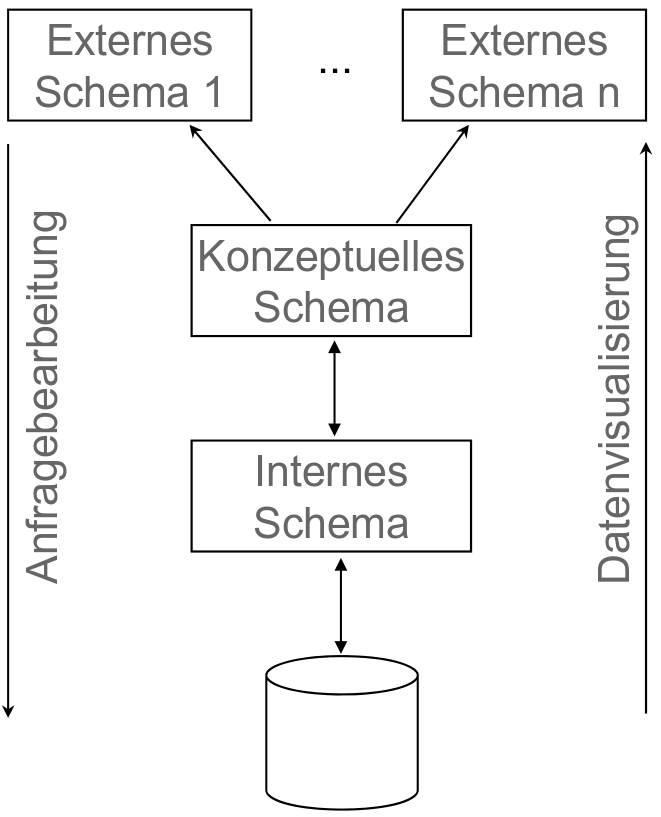
\includegraphics[width=0.15\textwidth]{DreiEbenenSchema}\end{figure}
\begin{itemize}
  \item \textbf{Konzeptionelles Schema}: Diskursbereich? Welche Entitäten interessant (bei Studierenden Noten interessant, Hobbies usw. nicht)?
  \item \textbf{Internes Schema}: physische Datenrepräsentation
  \item \textbf{Externe Schemata}: Unterschiedlicher Datenausschnitt für unterschiedliche Nutzer (Datenschutz, Übersichtlichkeit, organisatorische Gründe, Verstecken von Änderungen am konzeptionellen Schema)
  \item \( \leadsto \) \emph{Logische Datenunabhängigkeit}
\end{itemize}



\paragraph{Datenbankprinzipien --- Coddsche Regeln}
\begin{itemize}
  \item \textbf{Integration}: Einheitliche, nichtredundante Datenverwaltung
  \item \textbf{Operationen}: Speichern, Suchen, Ändern
  \item \textbf{Katalog}: Zugriff auf Datenbankbeschreibungen im data directory
  \item \textbf{Benutzersichten}
  \item \textbf{Integritätssicherung}: Korrektheit des DB-Inhalts
  \item \textbf{Datenschutz}: Ausschluss unauthorisierter Zugriffe
  \item \textbf{Transaktionen}: mehrere DB-Operationen als Funktionseinheit (= Atomarität)
  \item \textbf{Synchronisation}: parallele Transaktionen koordinieren (= Isolation)
  \item \textbf{Datensicherung}: Wiederherstellung von Daten nach Systemfehlern
  \item Strengste bekannte Datenbankdefinition
  \item Funktionale Anforderungen (nichtfunktional z.B.: Wie schnell/zuverlässig muss Dienst sein, kurze Antwortzeiten, Zuverlässigkeit, Effizienz, Skalierbarkeit)
\end{itemize}

\begin{fragen}
  \item Was ist eine Sicht?
  \item Was ist die relationale Algebra? Wozu braucht man sie?
  \item Geben Sie Beispiele für Algebra-Ausdrücke an, die nicht identisch, aber äquivalent sind, an.
  \item Was leistet der Anfragenoptimierer einer Datenbank?
  \item Erklären Sie: Drei-Ebenen-Architektur, physische/logische Datenunabhängigkeit.
\end{fragen}
  \section{Clustering und Ausreißer}
\label{sec:clustering}

\paragraph{Räumliche Indexstrukturen --- Motivation}
\begin{items}
	\item Was ist die nächste Bar, die mein bevorzugtes Bier ausschenkt?
	\item \textbf{Bereichsanfrage}: Wie viele Restaurants gibt es im Stadtzentrum?
	\item Ähnlichkeitssuche Bilder: Distanz im Merkmalsraum = Maß der Unähnlichkeit
	\item Ziel eines \textbf{Index}: Zahl der zu ladenden Seiten minimieren
\end{items}

\paragraph{Index --- B+-tree}
\begin{items}
	\item = non-clustered primary B+-tree
	\item Beispiel: Student(name, age, gpa, major), B+T für gpa \\* (kleiner=links, größer=rechts, (gpa, (Seite, Eintrag)))
	\begin{figure}[H]\centering\label{BPTree}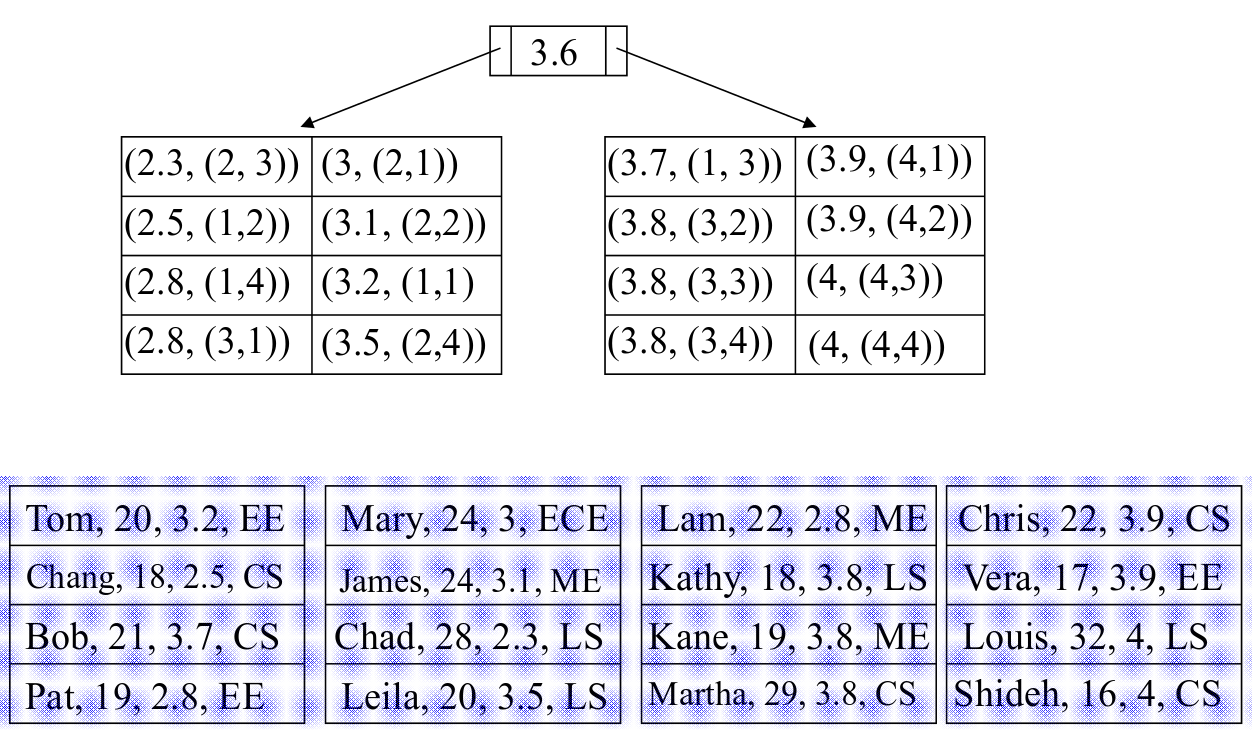
\includegraphics[width=0.33\textwidth]{BPTree}\end{figure}
\end{items}



\paragraph{Index --- kd-tree}
\begin{items}
	\item B+T löst Bar-Problem nicht wirklich
	\item kd-tree: Splitting für eine Dimension nach der anderen, dann wieder von vorne
	\item Beispiel: Vier Split-Dimensionen
\end{items}
\begin{figure}[H]\centering\label{KDTree}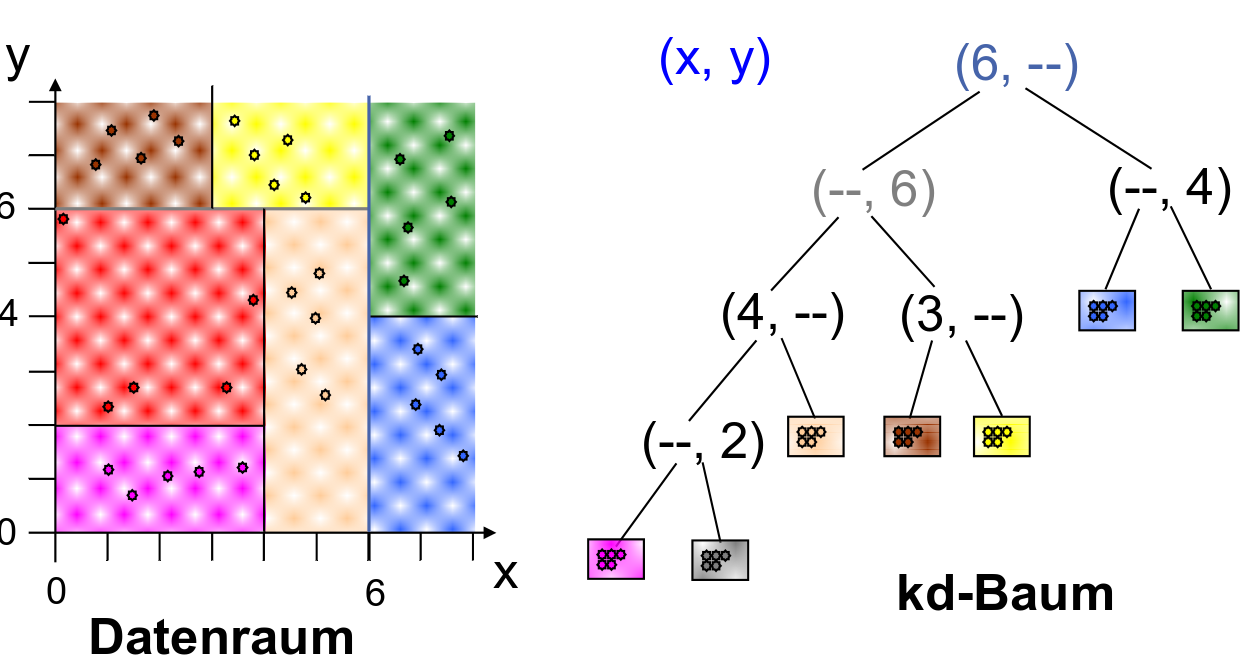
\includegraphics[width=0.33\textwidth]{KDTree}\end{figure}

\paragraph{kd-tree --- k-NN}
\begin{items}
	\item k-NN (= \emph{k-next-neighbour}) := Abstand des \( k \)-nächsten Nachbarn
	\item Es müssen nur ein paar kd-Baum-Regionen inspiziert werden, um Resultat zu ermitteln (Abstand zu Region ist untere Schranke)
	\item \textbf{Implementierung}: Priority Queue (Datenobjekte/Baumknoten, sortiert nach Abstand zum Anfragepunkt) initialisiert mit Wurzelknoten; Vorderstes Objekt aufspalten und Teilobjekte einfügen; Ende wenn Punkt vorne in Queue
	\item Hier: Baum unbalanciert, Balancierung in Realität für mehrdimensionale Daten
\end{items}

\paragraph{Outlier}
\begin{items}
	\item Element des Datenbestands, das in bestimmter Hinsicht erheblich vom restlichen Datenbestand abweicht
	\item Mögliche Definition: \\*
		Objekt \( O \), das in Datenbestand \( T \) enthalten ist ist ein DB(\( p \), \( D \))-Outlier, wenn der Abstand von \( O \) zu mindestens \( p \) Prozent der Objekte in \( T \) größer ist als \( D \).
	\item \textbf{Beispiel}: \( O \) ist Outlier, wenn \( p=0.6 \), da dann mehr als \( 60\% \) der Datenobjekte außerhalb des Kreises liegen
\end{items}
\begin{figure}[H]\centering\label{Outlier}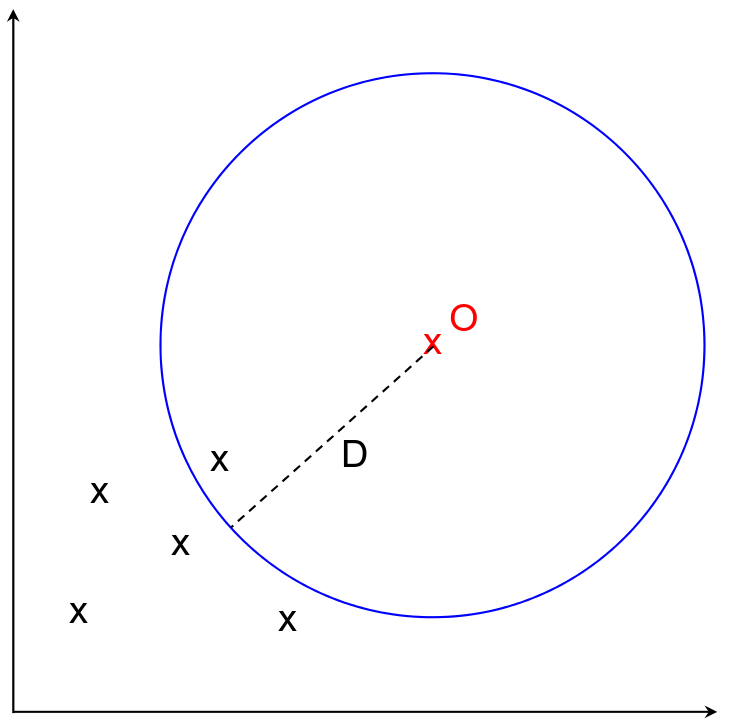
\includegraphics[width=0.2\textwidth]{Outlier}\end{figure}

\paragraph{Outlier --- Index-basiert}
\begin{items}
	\item Punkt ist kein Outlier, wenn k-Abstand < D mit $k = N * (1 - p) - 1$
	\item Für jeden Punkt:\\*
		k-NN Query, dabei stoppen sobald größte noch mögliche k-NN Distanz < D  (Baumknoten mit k Objekten und größter Distanz < D)
	\item Viele weitere Ansätze, z.B. \\*
		\textbf{Clustering}: Liefert Outlier als Beiprodukt
\end{items}



\paragraph{Clustering --- Beispiel Customer Segmentation}
\begin{items}
	\item Große Kundendatenbank mit Eigenschaften und Käufen
	\item Gesucht: Gruppen von Kunden mit ähnlichem Verhalten finden
\end{items}

\paragraph{Clustering --- DBSCAN}
\begin{items}
	\item \textbf{Dichte}: Anzahl Objekte pro Volumeneinheit
	\item \textbf{Dichtes Objekt}: mindestens \( x \) andere Objekte in Kugel um Objekt mit Radius \( \epsilon \) (A)
	\item \textbf{Dichte-erreichbares Objekt}: Objekt in \( \epsilon \)-Umgebung eines dichten Objekts, das selbst nicht dicht ist (B, C) \\*
		Clusterrand, Zuordnung zu Clustern ist nichtdeterministisch
	\item \textbf{Rauschen} (\emph{Noise}): Objekte, die von keinem dichten Objekt erreicht werden können (N)
\end{items}
\begin{figure}[H]\centering\label{DBSCAN}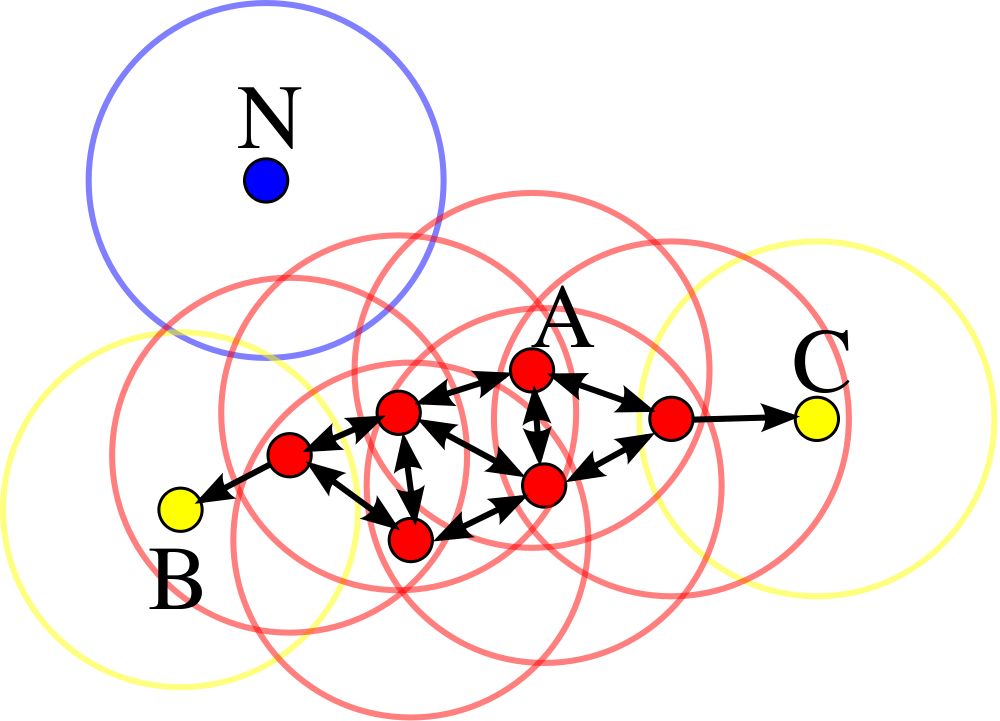
\includegraphics[width=0.2\textwidth]{DBSCAN}\end{figure}

\paragraph{DBSCAN --- Eigenschaften}
\begin{items}
	\item \textbf{Komplexität}: Lineare, wenn \( \epsilon \)-Umgebungen vorberechnet wurden (oder mit räumlichem Index in konstanter Zeit bestimmt werden können) \\* \( \leadsto \) mehrdimensionale Indexstruktur sehr sinnvoll
	\item Rauschen liefert \emph{mögliche} Outlier (DBSCAN erstellt Vorauswahl)
\end{items}

\paragraph{Hochdimensionale Datenräume --- Anomalien}
\begin{items}
	\item Curse of dimensionality
	\item \textbf{Sparsity}: Raum ist nur dünn mit Punkten besetzt
	\item Hierarchische Datenstrukturen ineffektiv: Es müssen immer alle Blätter betrachtet werden
	\item Keine echten Outlier: bei sehr, sehr vielen Dimensionen ist Abstand zweier Datenobjekte fast gleich dem zweier anderer \( \leadsto \) Outlier-Algorithmen liefern mehr oder weniger zufälliges Objekt
	\item \( \leadsto \) nur erfolgsversprechende Teilräume nach Ausreißern absuchen
	\item Interessante Cluster sind i.d.R. nicht Cluster in allen Dimensionen
\end{items}

\paragraph{Outlier --- im Höherdimensionalen}
\begin{items}
	\item Outlier erscheinen als solche nur in Teilräumen
	\item Manche Teilräume ausreißerfrei
	\item Unterschiedlichdimensionale Teilräume enthalten Ausreißer
	\item trivial vs. nichttrivial: \\*
		- \emph{trivial}: Objekt ist in Teilraum bereits Ausreißer \\*
		- \emph{nichttrivial}: Gegenteil
	\item \( \leadsto \) Maß für Teilraumrelevanz --- wie findet man relevante TR?
\end{items}

\paragraph{Subspace Search}
\begin{items}
	\item Exponentiell viele Teilräume \( P(A) \)
	\item Auswahl relevanter Teilräume \( RS \subset P(A) \)
\end{items}

\paragraph{HiCS --- Prinzip}
\begin{items}
	\item Attribute korrelieren nicht \( \leadsto \) Outlier in diesem Raum tendenziell eher trivial
	\item \textbf{Idee}: Suche nach Verletzung statistischer Unabhängigkeit \\* (= \emph{Kontrast})
\end{items}

\begin{fragen}
	\item Warum kann man räumliche Anfragen nicht ohne Weiteres auswerten, wenn man für jede Dimension separat einen B-Baum angelegt hat?
	\item Wie funktioniert der Algorithmus für die Suche nach den \( k \) nächsten Nachbarn mit Bäumen wie dem kd-Baum?
	\item Warum werden bei der NN-Suche nur genau die Knoten inspiziert, deren Zonen die NN-Kugel überlappen?
	\item Was ist ein Outlier?
	\item Was ist ein Zusammenhang zwischen \( k \)-NN-Suche mit Bäumen wie dem kd-Baum und Outlier-Berechnung?
	\item Warum ist die Zuordnung Dichte-erreichbarer Punkte mit DBSCAN nichtdeterministisch?
	\item Warum sind hierarchische Datenstrukturen in hochdimensionalen Merkmalsräumen für die \( k \)-NN-Suche nicht das Mittel der Wahl?
	\item Was bedeutet \emph{Subspace Search}?
	\item Geben Sie die Unterscheidung zwischen trivialen und nichttrivialen Outliern aus der Vorlesung wieder.
	\item Was genau bedeutet \emph{Kontrast} im Kontext von HiCS?
\end{fragen}
  \section{Datenbank-Definitionssprachen}
\label{sec:definitionssprachen}

\paragraph{Gewinnung der Konventionen}
\begin{items}
	\item Beschränkte Anwendungswelt (= Miniwelt, relevanter Weltausschnitt, Diskursbereich)
	\item \textbf{Daten}: Modelle (gedankliche Abstraktionen) der Miniwelt
	\item \textbf{Datenbasiskonsistenz}: Datenbasis ist bedeutungstreu, wenn ihre Elemente Modelle einer gegebenen Miniwelt sind (schärfste Konsistenzforderung)
\end{items}

\paragraph{Datenbankentwurf --- Phasenmodell}
\begin{figure}[H]\centering\label{Phasenmodell}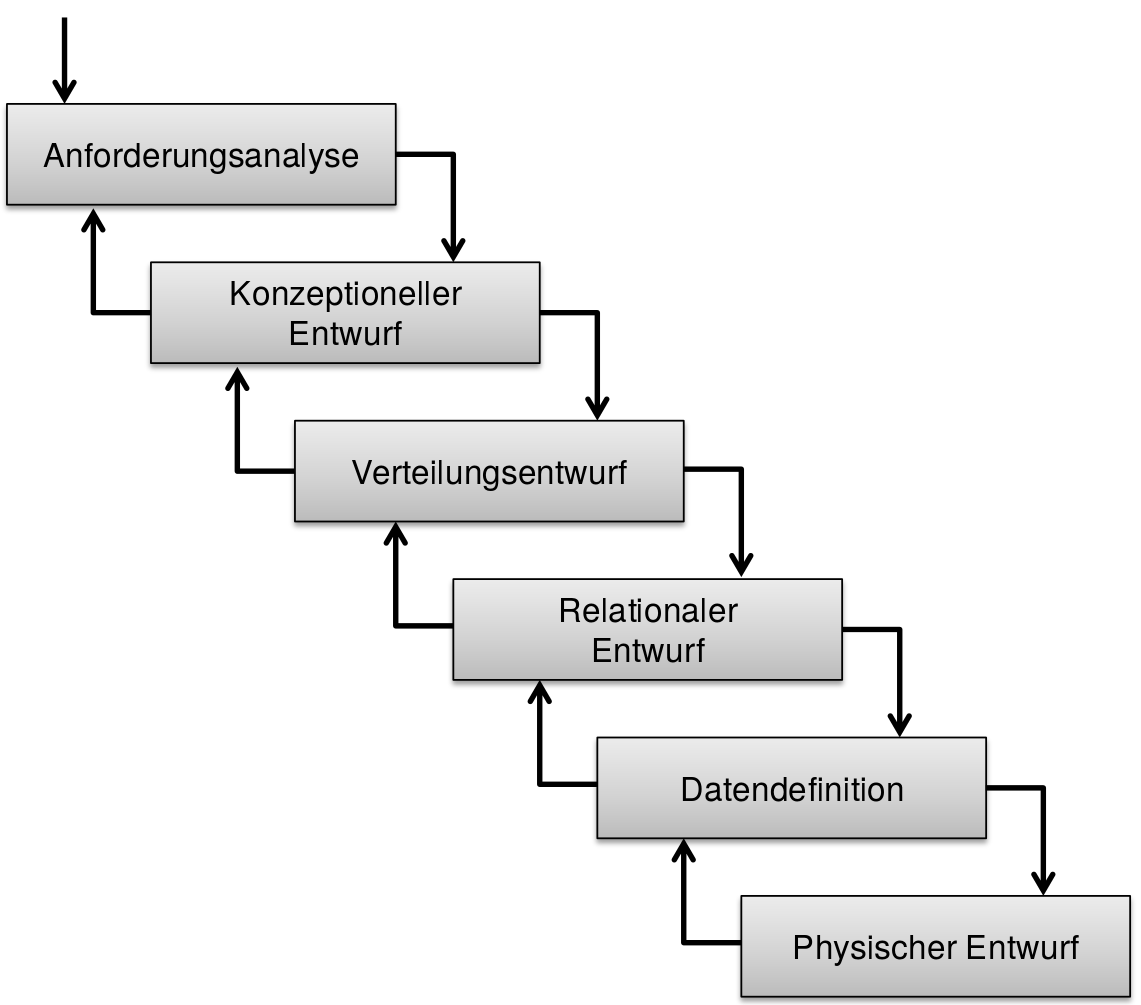
\includegraphics[width=0.33\textwidth]{Phasenmodell}\end{figure}

\paragraph{Datenbankentwurf --- Modellierung}
\begin{items}
	\item Ausschnitt der Wirklichkeit mit Schema beschreiben
	\item Typen = Struktur der Entitäten
	\item Welche Konsistenzbedingungen sind sinnvoll?
	\item \textbf{Schemakonsistenz}: Einhaltung der durch Schema vorgegebenen Konsistenzbedingungen (= von DBMS überprüfbar! )
\end{items}

\paragraph{SQL}
\begin{items}
	\item = standardisierte Sprache für DB-Zugriff (relational)
	\item Aspekte: \\*
		- Schemadefinition \\*
		- Datenmanipulation (Einfügen, Löschen, Ändern) \\*
		- Anfragen
\end{items}



\paragraph{SQL --- SQL-DDL}
\begin{items}
	\item = \emph{SQL data definition language}
	\item Teilbereich von SQL, der zu tun hat mit Definition von: \\*
		- Typen \\*
		- Wertebereichen
		- Relationsschemata \\*
		- Integritätsbedingungen
\end{items}

\paragraph{SQL --- als Definitionssprache}
\begin{items}
	\item Externe Ebene: 
		\begin{lstlisting}[language=sql]
{ create | drop } view;
		\end{lstlisting}
	\item Konzeptuelle Ebene:
		\begin{lstlisting}[language=sql]
{ create | alter | drop } table;
{ create | alter | drop } domain;
		\end{lstlisting}
	\item Interne Ebene:
			\begin{lstlisting}[language=sql]
{ create | alter | drop } index;
		\end{lstlisting}
\end{items}

\paragraph{Data Dictionary}
\begin{items}
	\item Verzeichnis der vorhandenen Tabellen und Sichten
	\item Selbst wie eine Datenbank aufgebaut
	\item Enthält keine Anwendungsdaten, sondern Struktur-Metadaten
\end{items}

\paragraph{SQL --- Tabelle anlegen}
\begin{items}
	\item \begin{lstlisting}[language=sql]
create table Kuenstler
  (KID integer, NAME varchar(200), 
   LAND varchar(50) not null, JAHR integer, 
   primary key (KID))
\end{lstlisting}
\end{items}

\paragraph{SQL --- Wertebereiche}
\begin{items}
	\item \lstinline[language=sql]{integer} (auch \lstinline[language=sql]{int})
	\item \lstinline[language=sql]{smallint}
	\item \lstinline[language=sql]{float(p)} (auch \lstinline[language=sql]{float})
	\item \lstinline[language=sql]{decimal(p,q)} (auch \lstinline[language=sql]{numeric(p,q)}, jeweils mit \lstinline[language=sql]{q} Nachkommastellen)
	\item \lstinline[language=sql]{character(n)} (auch \lstinline[language=sql]{char(n)} oder \lstinline[language=sql]{char} für \( n=1 \))
	\item \lstinline[language=sql]{character varying(n)} (auch \lstinline[language=sql]{varchar(n)}, String variabler Länge bis Maximallänge \( n \))
	\item \lstinline[language=sql]{bit(n)} (oder \lstinline[language=sql]{varying(n)} analog für Bitfolgen)
	\item \lstinline[language=sql]{date}, \lstinline[language=sql]{time}, \lstinline[language=sql]{timestamp}
\end{items}

\paragraph{Wertebereiche --- Custom}
\begin{items}
	\item \begin{lstlisting}[language=sql]
create domain Gebiete varchar(20)
  default 'Informatik'
\end{lstlisting}
	\item \begin{lstlisting}[language=sql]
create table Vorlesungen
  (Bezeichnung varchar(80) not null, SWS smallint,
   Semester smallint, Studiengang Gebiete)
\end{lstlisting}
\end{items}

\paragraph{Integritätsbedingungen}
\begin{items}
	\item Schlüssel kann aus mehreren Attributen bestehen
	\item \textbf{Fremdschlüssel}: \begin{lstlisting}[language=sql]
create table Titel
  (TITLEID integer not null, NAME varchar(200), 
   KID integer, primary key (TITLEID), 
   foreign key (KID) references Kuenstler(KID))
\end{lstlisting}
	\item \lstinline[language=sql]{default}-Klausel: Standardwert für Attribut
	\item \lstinline[language=sql]{check}-Klausel: weitere lokale Integritätsbedingungen
	\item \begin{lstlisting}[language=sql]
create table Vorlesungen
  (Bezeichnung varchar(80) not null, SWS smallint,
   Semester smallint, check(Semester between 1 and 9), 
   Studiengang Gebiete)
\end{lstlisting}
\end{items}



\paragraph{SQL --- alter und drop}
\begin{items}
	\item \begin{lstlisting}[language=sql]
alter table Lehrstuehle
  add Budget decimal(8,2)
  add constraint Namekey primary key (Name, Vorname)
\end{lstlisting}
	\item \( \leadsto \) Änderung Relationsschema im Data Dictionary, existierende Daten werden um \lstinline[language=sql]{null}-Attribut erweitert
	\item \begin{lstlisting}[language=sql]
drop spaltenname { restrict | cascade }
drop table basisrelationenname { restrict | cascade }
\end{lstlisting}
\item \( \leadsto \) Attribut / Tabelle löschen, dabei gilt: \\*
	- \lstinline[language=sql]{restrict}: keine Sichten/Integritätsbedingungen mit diesem Attribut definiert wurden \\*
	- \lstinline[language=sql]{cascade}: gleichzeitig diese Schichten/Integritätsbedingungen mitgelöscht werden sollen
\end{items}

\paragraph{Speicherhierarchie}
\begin{figure}[H]\centering\label{Speicherhierarchie}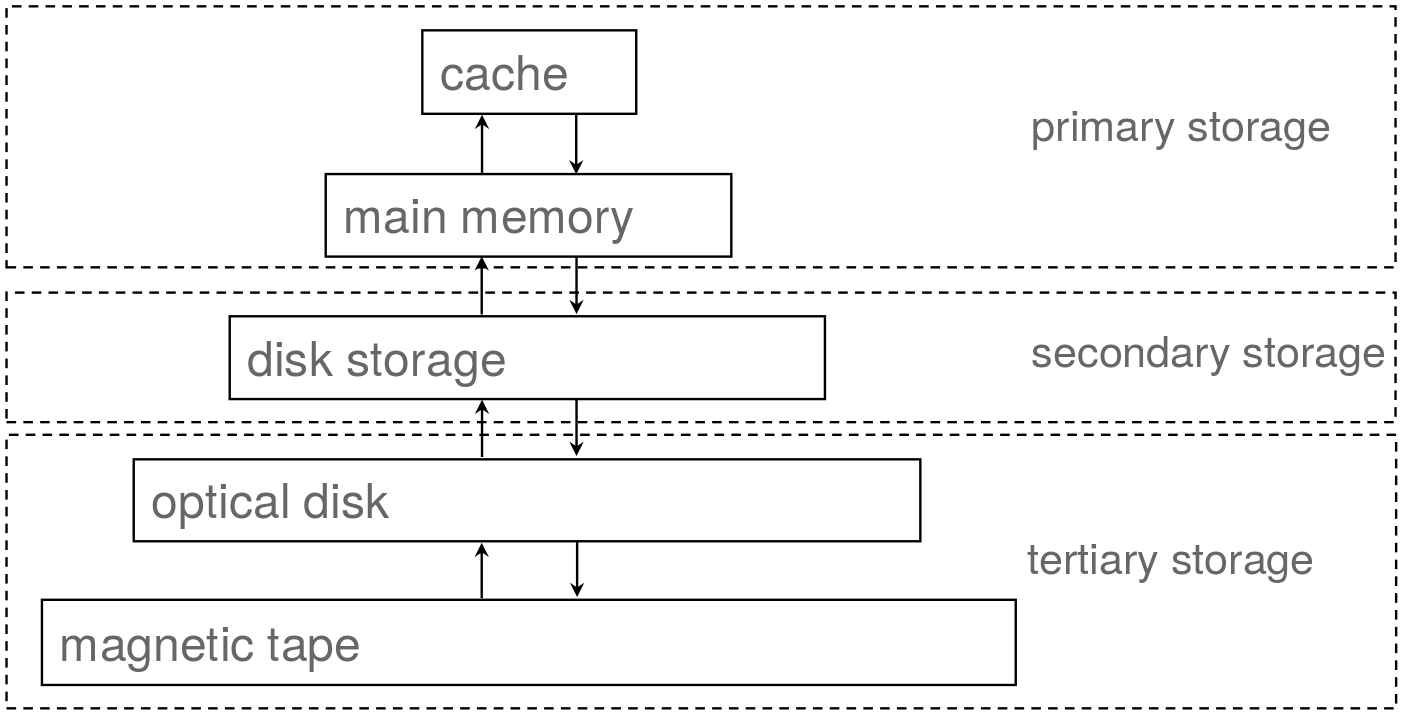
\includegraphics[width=0.33\textwidth]{Speicherhierarchie}\end{figure}

\paragraph{Index}
\begin{items}
	\item Für mehrere Attribute möglich
	\item Index für (gpa, name) \( \neq \) Index für (name, gpa)
	\item Index kann nachträglich angelegt bzw. gelöscht werden, ohne Daten selbst zu löschen
	\item Index Bestandteil der physischen Ebene, Index-Definition Teil des internen Schemas
	\item \lstinline[language=sql]{select name from Student where gpa > 4} liefert Ergebnis unabhängig von Existenz eines Index --- wenn vorhanden erhebliche Beschleunigung
	\item \lstinline[language=sql]{create [unique] index typ on auto(hersteller, modell, baujahr)} \\* hilft bei Herstellersuche, weniger bei Suche nach Baujahr
	\item Unique Index zur Simulation von Schlüsselbedingungen
\end{items}
\begin{figure}[H]\centering\label{Index}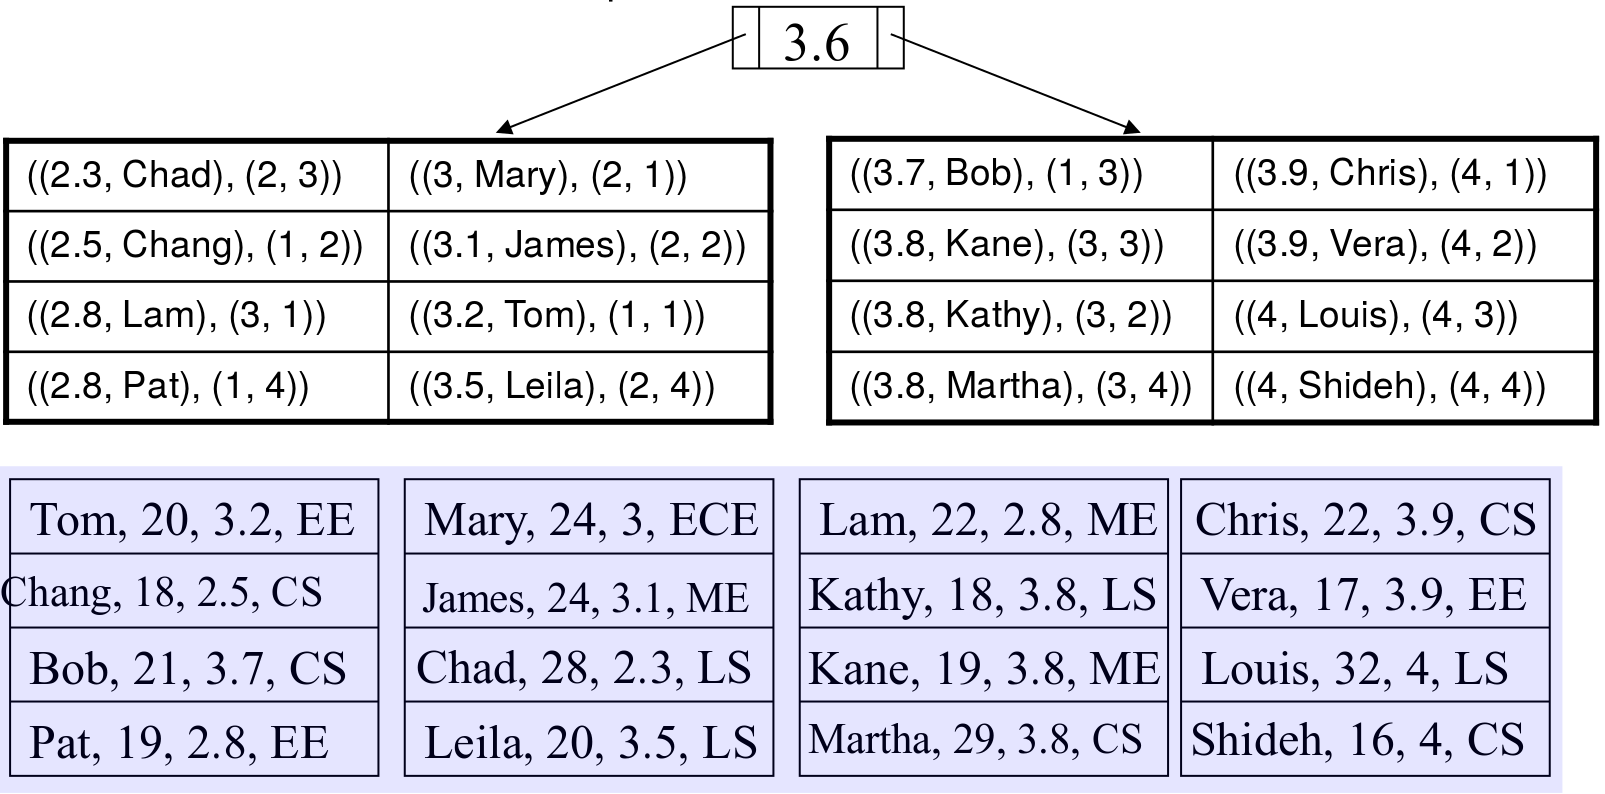
\includegraphics[width=0.33\textwidth]{Index}\end{figure}

\begin{fragen}
	\item Erläutern Sie anhand eines Anwendungsbeispiels, warum man die Menge der zulässigen Zustände einschränken will.
	\item Was ist Schema-Konsistenz, Datenbasis-Konsistenz?
	\item Was ist ein (DB-)Schema?
	\item Was ist das Data Dictionary?
	\item Warum sollte man sich die Mühe machen, Integritätsbedingungen als Teil des DB-Schemas zu formulieren?
	\item Sind Integritätsbedingungen Bestandteil des internen oder des konzeptuellen Schemas? Begründen Sie Ihre Antwort.
	\item Wieso sind Indices Bestandteil des internen und nicht des konzeptuellen Schemas?
	\item Geben Sie Beispiele für DB-Features an, die zeigen, dass DB-Systeme physische Datenunabhängigkeit nicht vollständig umsetzen.
\end{fragen}
  \section{Datenbankmodelle für den Entwurf}
\label{sec:entwurf}

\paragraph{Entity-Relationship-Modelle}
\begin{items}
	\item \textbf{Entity}: Objekt der Real-/Vorstellungswelt (z.B. Buch)
	\item \textbf{Relationship}: Beziehung zw. Entities (z.B. Schüler hat Buch)
	\item \textbf{Attribut}: Eigenschaft von Entities (z.B. ISBN)
\end{items}
\begin{figure}[H]\centering\label{EntityRelationship}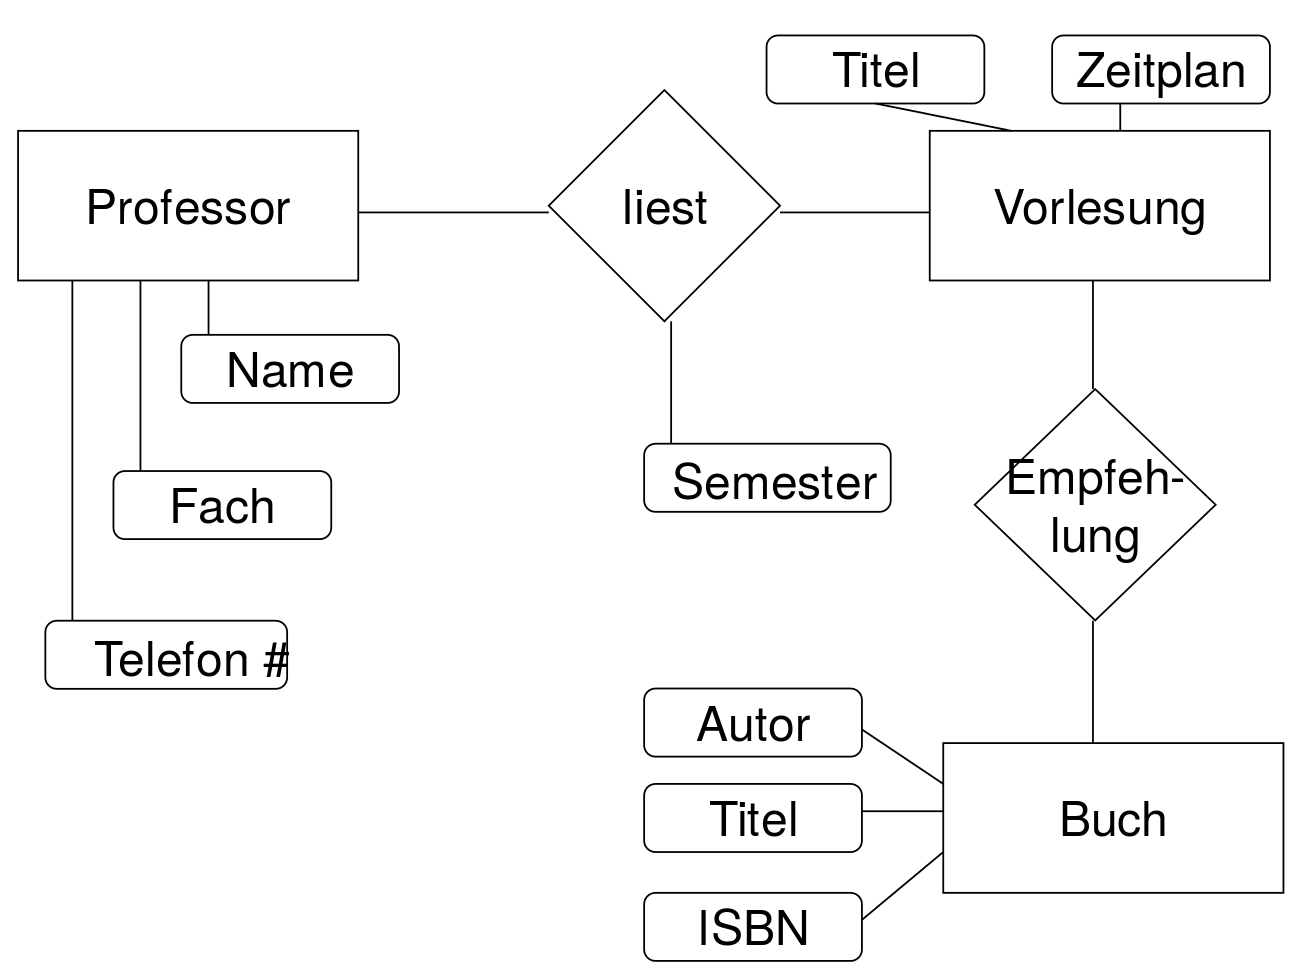
\includegraphics[width=0.33\textwidth]{EntityRelationship}\end{figure}

\paragraph{Attribute}
\begin{items}
	\item \textbf{Mengenwertig:} Durch Doppelrand gekennzeichnet
	\item \textbf{Optional:}
	\begin{figure}[H]\centering\label{OptionaleAttribute}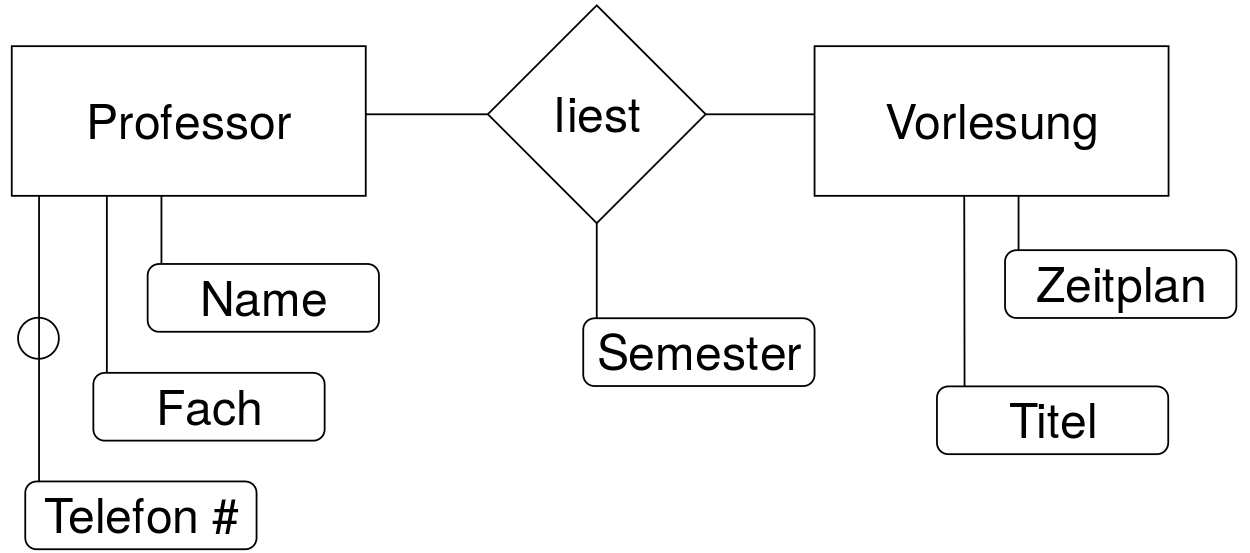
\includegraphics[width=0.33\textwidth]{OptionaleAttribute}\end{figure}
\end{items}

\paragraph{ER --- Modellierungskonzepte}
\begin{items}
	\item \( \mu(D) \): Interpretation von \( D \), mögliche Werte einer Entity-Eig.
	\item \( \mu \)(\lstinline[language=sql]{int}): \( \mathbb{Z} \),  \( \mu \)(\lstinline[language=sql]{string}): \( C^\star \) (Folgen von Zeichen aus \( C \))
	\item \( \mu(E) \): Menge der möglichen Entities vom Typ \( E \)
	\item \( \sigma_i \)(E): Menge der \emph{aktuellen} Entities vom Typ \( E \) in Zustand \( \sigma\)
	\\* \( \leadsto \) \( \sigma(E) \subseteq \mu(E) \) und \( \sigma(E) \) endlich
	\item \( \mu(R) = \mu(E_1) \times \cdots \times \mu(E_n) \) \\* \( \leadsto \) Die Menge aller möglichen Ehen ist die Menge aller (Mann,Frau)-Paare.
	\item \( \sigma(R) \subseteq \sigma(E_1) \times \cdots \times \sigma(E_n) \) \\* \( \leadsto \) aktuelle Beziehungen nur zwischen aktuellen Entities
	\item Attribut \( A \) eines Entity-Typen \( E \) ist im Zustand \( \sigma \) eine Abbildung \( \sigma(A): \sigma(E) \to \mu(D) \) (\textbf{nicht} \( A: \sigma(E) \to \mu(D) \))
	\item Beziehungsattribute: \( \sigma(A): \sigma(R) \to \mu(D) \) (Beziehung \( R \), Attribut \( A \), möglicher Wertebereich \( \mu(D) \))
\end{items}

\paragraph{Mehrstellige Beziehungen}
\begin{items}
	\item Umwandlung von mehrstelligen Beziehungen in mehrere einstellige Beziehungen i.A. nicht einfach möglich.
\end{items}

\paragraph{Funktionale Beziehungen}
\begin{items}
	\item Jedem Professor lässt sich ein Zimmer zuordnen, umgekehrt nicht zwingend
	\item Schreibe: \( R: E_1 \to E_2 \)
\end{items}
\begin{figure}[H]\centering\label{FunktionaleBeziehung}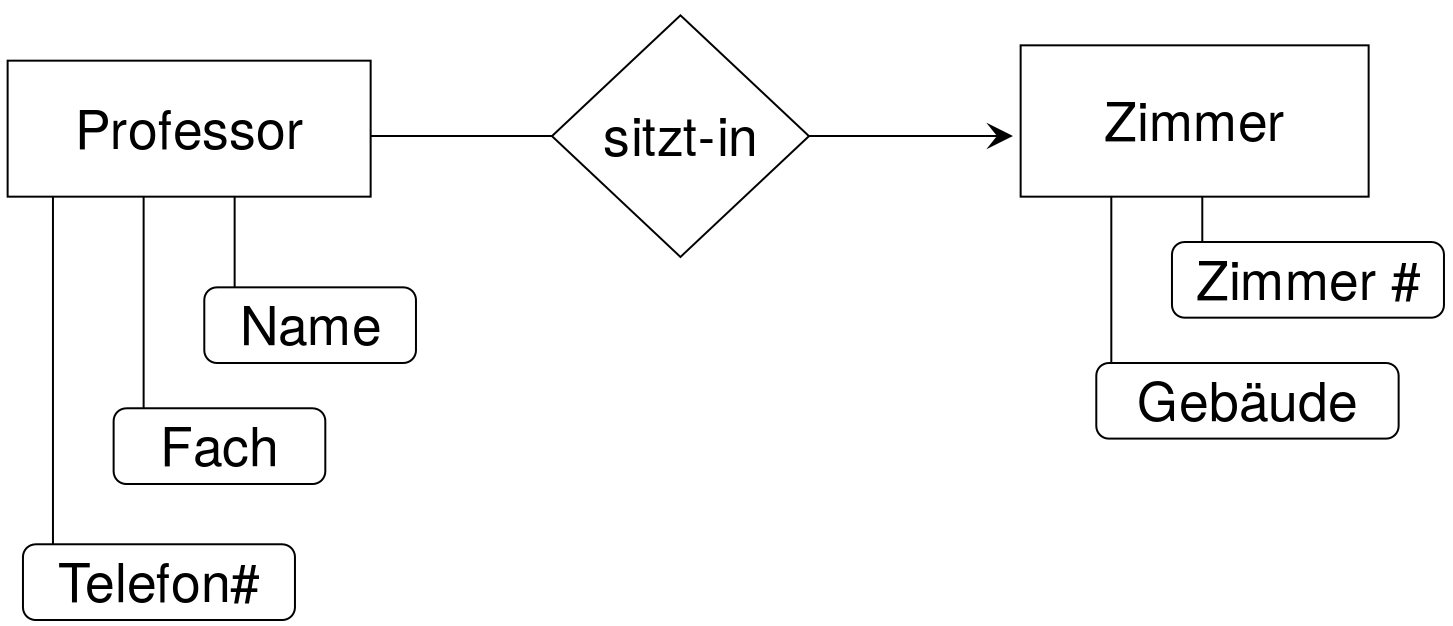
\includegraphics[width=0.33\textwidth]{FunktionaleBeziehung}\end{figure}



\paragraph{Schlüssel}
\begin{items}
	\item Schlüsselattribute \( \{ S_1, \dots, S_k \} \subseteq \{ A_1, \dots, A_m \} \) für \\* Entity-Typ \( E(A_1, \dots, A_m) \)
	\item Notation: Schlüssel unterstreichen: \( E(\dots, \underline{S_1}, \dots, \underline{S_i}, \dots) \)
	\item Schlüssel ist minimal: Wird ein Schlüsselattribut entfernt, so ist das entstehende Tupel nicht mehr eindeutig
\end{items}

\paragraph{Abhängige Entity-Typen}
\begin{items}
	\item Identifikation über funktionale Beziehung (als Schlüssel)\\
	Bsp: (Exemplar-)Nummer bezieht sich auf jeweiliges Buch
\end{items}
\begin{figure}[H]\centering\label{AbhaengigeEntity}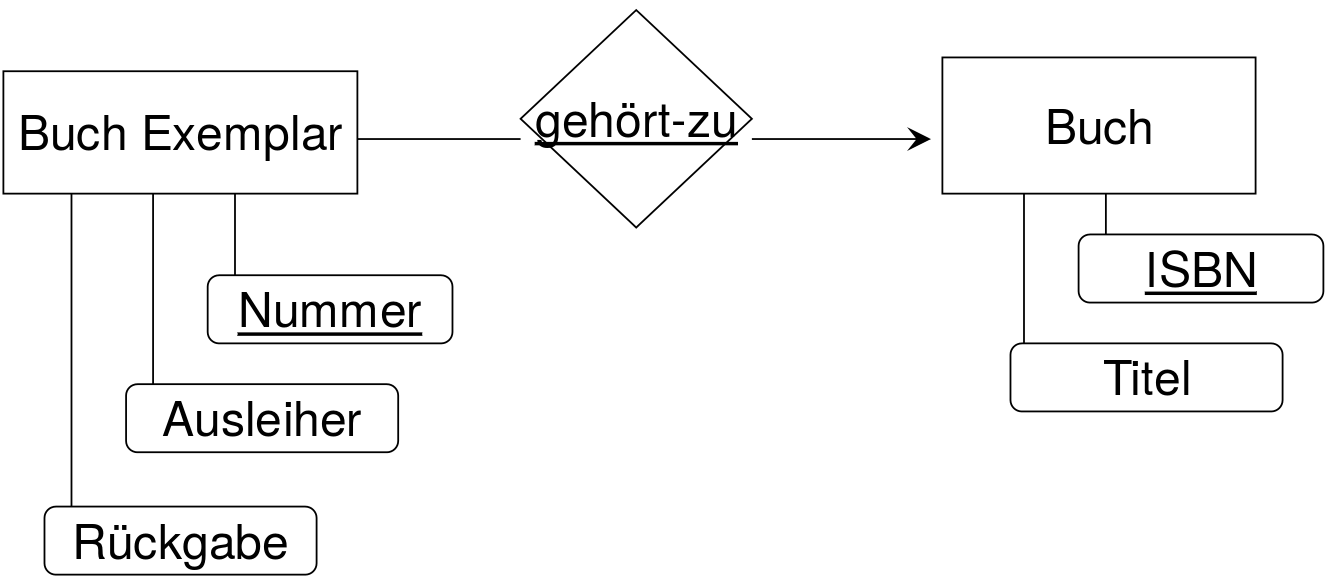
\includegraphics[width=0.33\textwidth]{AbhaengigeEntity}\end{figure}

\paragraph{IST-Beziehung}
\begin{figure}[H]\centering\label{ISTBeziehung}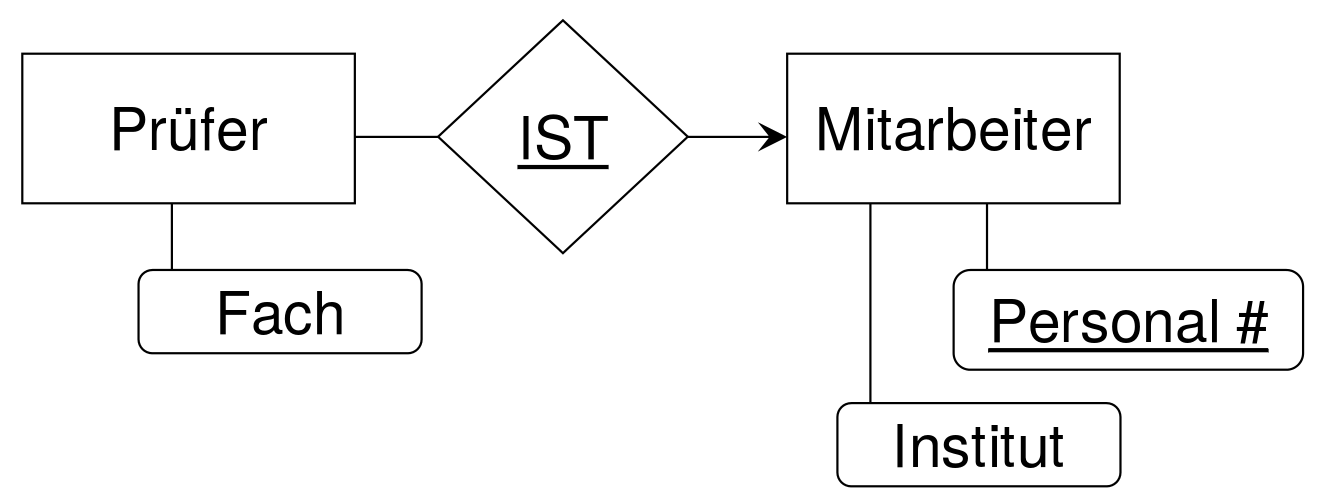
\includegraphics[width=0.33\textwidth]{ISTBeziehung}\end{figure}
\begin{items}
	\item Spezialfall eines abhängigen Entity-Typen (nur Beziehung als Schlüssel)
	\item Vererbung von Attributen (und Werten): \\* \( \sigma(\text{Prüfer}) \subseteq \sigma(\text{Mitarbeiter}) \)
\end{items}
\begin{figure}[H]\centering\label{MehrereFaecher}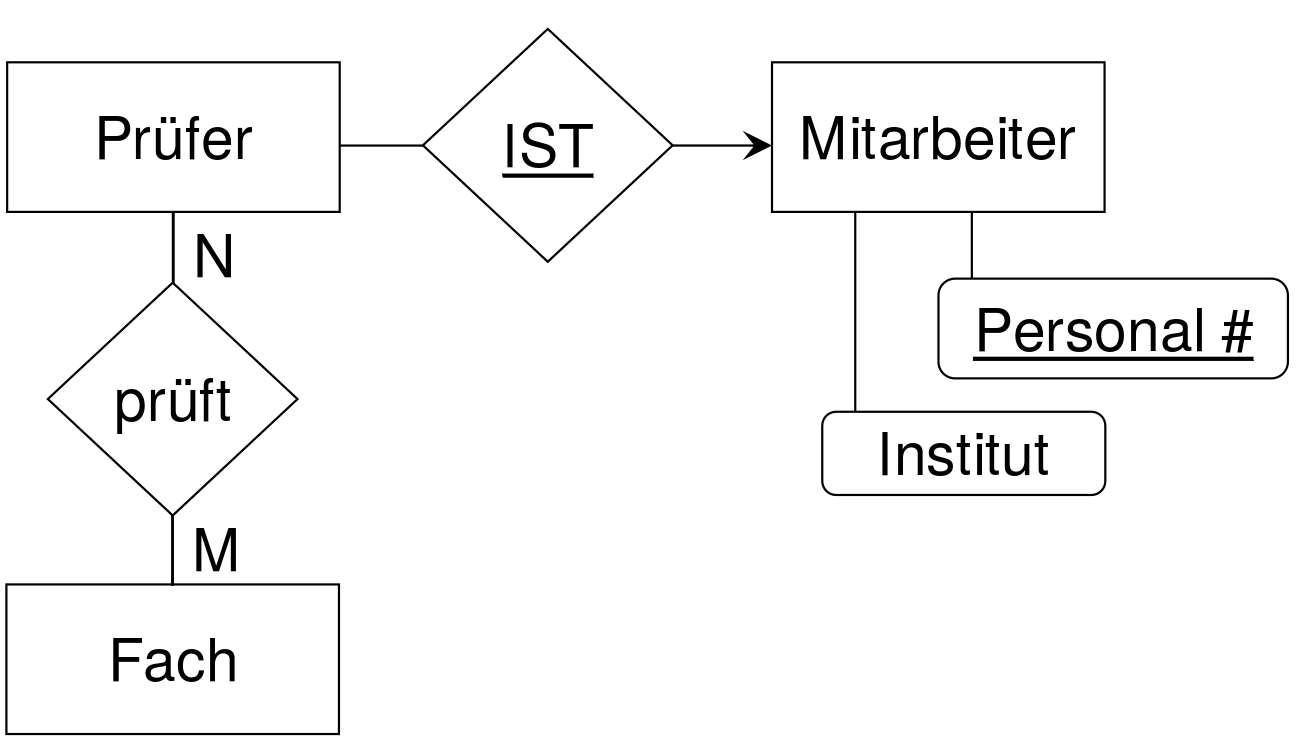
\includegraphics[width=0.33\textwidth]{MehrereFaecher}\end{figure}

\paragraph{Entwurf --- Kardinalitäten}
\begin{items}
	\item An wv. Beziehungen muss Entity teilnehmen? \( \leadsto \) einschränken
	\item \textbf{Teilnehmerkardinalität}: \lstinline[language=sql]{arbeitet_in(Mitarbeiter[0,1],Raum[0,3])} \\*
		- jeder Mitarbeiter hat einen oder keinen zugeordneten Raum \\*
	 	- pro Zimmer arbeiten maximal drei Mitarbeiter \\*
	 	- ein Zimmer kann leerstehen
	 \item \textbf{Standardkardinalität}: 1 Mannschaft steht mit 11 Spielern in Bezug \\*
	 Auch hier Intervallangabe möglich\\*
	  Speziell: \lstinline[language=sql]{m:n}/\lstinline[language=sql]{1:n}/\lstinline[language=sql]{1:1}-Beziehung (Untere Schranke jeweils \emph{0})
	 \begin{figure}[H]\centering\label{Mannschaft}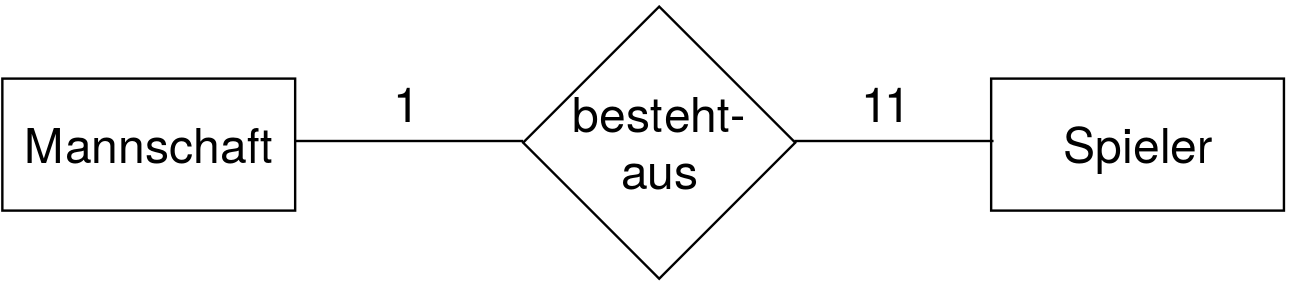
\includegraphics[width=0.33\textwidth]{Mannschaft}\end{figure}
\end{items}





\paragraph{Semantische Beziehungen}
\begin{items}
	\item \textbf{Spezialisierung}: \lstinline[language=sql]{Pruefer} Spezialisierung von \lstinline[language=sql]{Mitarbeiter} \\* \( \leadsto \) Vererbung (IST-Beziehung)
	\item \textbf{Partitionierung}: Spezialfall der Spezialisierung, mehrere \emph{disjunkte} Entity-Typen (z.B. Partitionierung von Buch in Monographie und Sammelband)
	\item \textbf{Generalisierung}: Buch oder DVD als Medium \\*
	\lstinline[language=sql]{Medium} ist stets \lstinline[language=sql]{DVD} oder \lstinline[language=sql]{Buch} \\* Aber: Buch muss kein Medium sein.
	\item \textbf{Aggregierung}: \lstinline[language=sql]{Auto} besteht aus \lstinline[language=sql]{Motor}, \lstinline[language=sql]{Karosserie},... \\* \( \leadsto \) Entity aus Instanzen anderer Entity-Typen zusammengesetzt
	\item \textbf{Sammlung} (auch Assoziation): \lstinline[language=sql]{Team} ist Gruppe von \lstinline[language=sql]{Person} \\* \( \leadsto \) Mengenbildung
\end{items}

\paragraph{EER}
\begin{items}
	\item = Erweitertes ER-Modell
	\item Übernommen: Werte, Entities, Beziehungen, Attribute, Funktionale Beziehungen, Schlüssel (jetzt ausgefüllter Kreis)
	\item Nicht übernommen: IST-Beziehung --- ersetzt durch \emph{Typkonstruktor}
\end{items}

\paragraph{EER --- Typkonstruktor}
\begin{items}
	\item Ermöglicht Spezialisierung, Generalisierung, Partitionierung
	\item Eingabetypen mit Dreiecksbasis verbunden (bei Generalisierung spezielle Typen, bei Spezialisierung/Partitionierung allgemeine Typen)
	\item Ausgabetypen mit Spitze verbunden
\end{items}
\begin{center}
	\begin{figure}[H]\centering\label{SpezialisierungEER}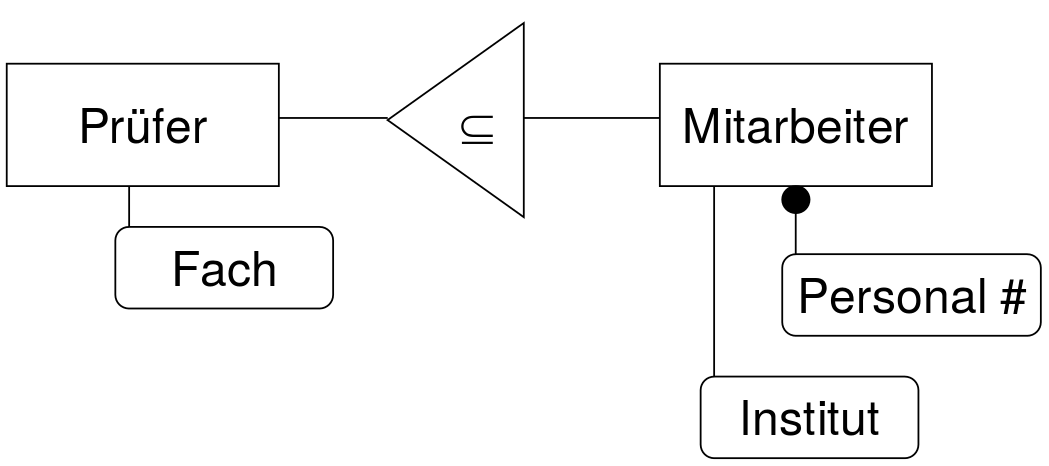
\includegraphics[width=0.33\textwidth]{SpezialisierungEER}\end{figure}
	Spezialisierung
	\begin{figure}[H]\centering\label{GeneralisierungEER}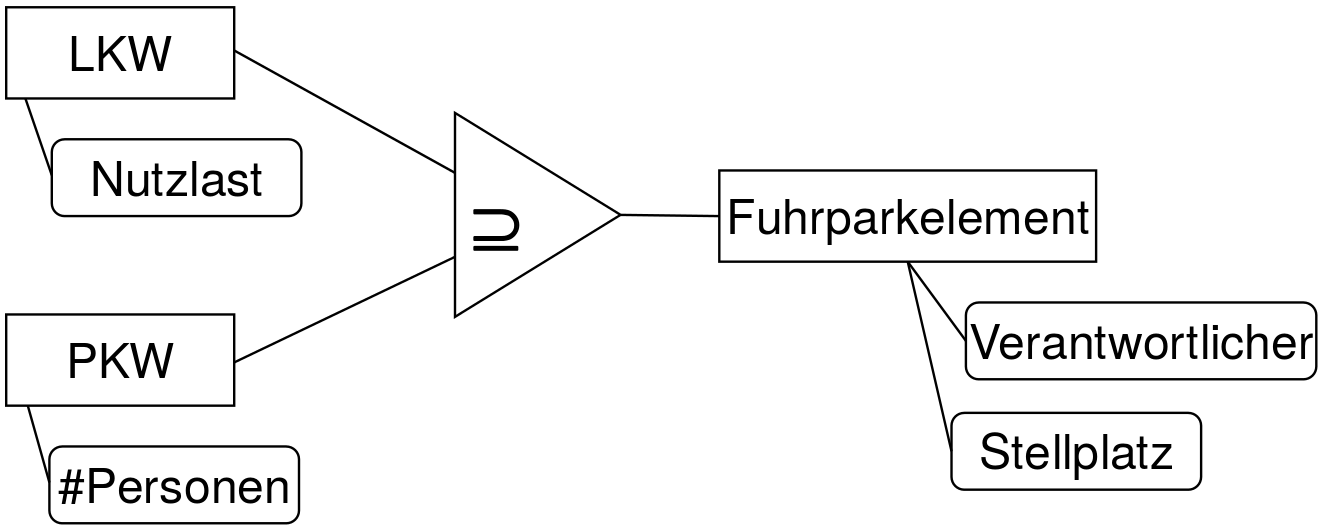
\includegraphics[width=0.33\textwidth]{GeneralisierungEER}\end{figure}
	Generalisierung
	\begin{figure}[H]\centering\label{MehrfacheSpezialisierungEER}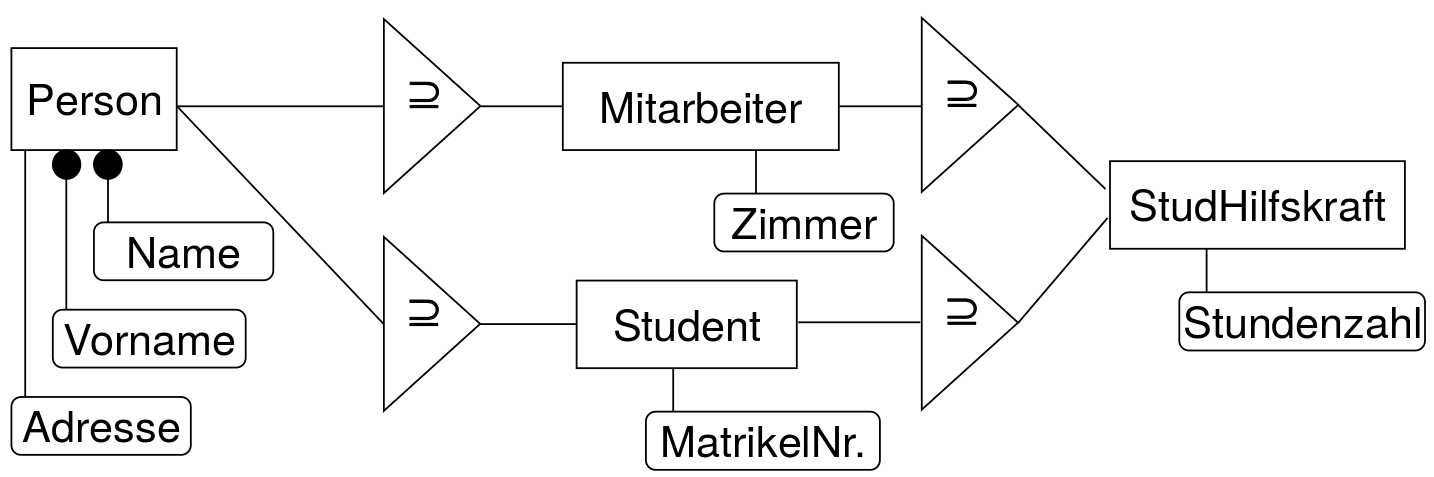
\includegraphics[width=0.33\textwidth]{MehrfacheSpezialisierungEER}\end{figure}
	Mehrfache Spezialisierung
\end{center}

\begin{fragen}
	\item Wie ist die Semantik von Datenmodellen definiert?
	\item Geben Sie ein Beispiel für mehrstellige Beziehungen an und erläutern Sie, warum der Sachverhalt mit mehreren zweistelligen Beziehungen nicht korrekt darstellbar wäre.
	\item Welche semantischen Beziehungen aus dem EER-Kontext kennen Sie? Erläutern Sie die Unterschiede und geben Sie jeweils ein Beispiel an.
\end{fragen}

  \section{Relationenentwurf}
\label{sec:relationenentwurf}

\paragraph{Formalisierung Relationenmodell}
\begin{itemize}
	\item \textbf{Universum} \( U \): nichtleere endliche Menge \( U \)\\* (z.B. \( U= \{ \text{Name}, \text{Alter}, \text{Haarfarbe}, \dots \} \))
	\item \textbf{Attribut}: \( A \in U \)
	\item \textbf{Domäne} \( D \in \{ D_1, \dots, D_m \} \): endliche, nichtleere Menge \\* (z.B. \( D_1 = \{ 1,2,3,\dots \}, D_2 = \{ \text{schwarz}, \text{rot}, \text{blond} \} \))
	\item \textbf{Attributwert}: \( w \in \text{dom}(A) \) Attributwert für \( A \), \( \text{dom}: U \to D \): total definierte Funktion, \( \text{dom}(A) \) Domäne von \( A \) \\* (z.B. \( \text{dom}(\text{Haarfarbe}) = \{ \text{schwarz}, \text{rot}, \text{blond} \} \))
	\item \textbf{Relationenschema}: \( R \subseteq U \)
	\item \textbf{Tupel} (\( t \) in \( R = \{ A_1, \dots, A_n \} \)): \( t: R \to \bigcup_{i=1}^n D_i \)
	\item \textbf{Relation} (\( r \) über \( R = \{ A_1, \dots, A_n \} \)): endliche Menge von Tupeln \\* Notation: \( r(R) \) (Relation \( r \), Relationenschema \( R \))
	\begin{figure}[H]\centering\label{BeispielRelation}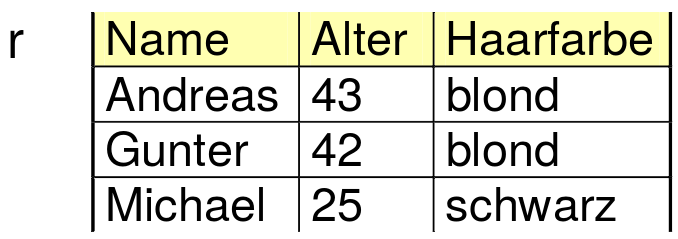
\includegraphics[width=.4\linewidth]{BeispielRelation}\end{figure}
	\item Beispiel: \\* \( R = \{ \text{Alter}, \text{Haarfarbe}, \text{Name} \} \) \\* \( r \) besteht aus Tupeln \( t_1, t_2, t_3 \); \( t_1(\text{Name}) = \text{``Andreas''} \) usw.
	\item \textbf{REL}: \( \text{REL}(R) = \{ r \mid r(R) \} \) \\* Menge aller Relationen über \( R \) sind \\* (\( r \) oben: \( r \in \text{REL}(\{ \text{Name}, \text{Alter}, \text{Haarfarbe} \}) \), \\* aber \( r \not \in \text{REL}(\{ \text{Name}, \text{Vorname} \}) \))
	\item \textbf{Datenbankschema}: \( S = \{ R_1, \dots, R_p \} \) \\* Menge von Relationenschemata
	\item \textbf{Datenbank} (\( d \) über \( S \)): Menge von Relationen \\* \( d = \{ r_1, \dots, r_p \} \) und \( r_i(R_i) \) \\* \( d(S) \) Datenbank \( d \) über \( S \)
\end{itemize}

\paragraph{Lokale Integritätsbedingung}
\begin{itemize}
	\item Abbildung aller möglichen Relationen zu einem Schema auf \lstinline{true} oder \lstinline{false}
	\item \( b: \text{REL}(R) \to \{ \) \lstinline{true}, \lstinline{false} \( \} \ (b \in B) \)
	\item \textbf{Erweitertes Relationenschema}: \( \mathcal{R} = (R, B) \)
	\item Abkürzung: \\* \( r(R) \) --- \( r \) ist Relation von \( R \) \\* \( r(\mathcal{R}) \) --- \( r \) ist Relation von \( R \), und \( b(r)= \) \lstinline{true} für alle \( b \in B \)
	\item \textbf{SAT}: \( \text{SAT}_R(B) = \{ r \mid r(\mathcal{R}) \} \) \\* Menge aller Relationen über erweitertem Relationenschema (SAT = \emph{satisfy})
\end{itemize}

\paragraph{Schlüssel}
\begin{itemize}
	\item Schlüssel und Fremdschlüssel einzige Integritätsbedingungen im relationalen Modell
	\item Schlüssel: Minimale identifizierende Attributmenge
	\item i.A. mehrere Schlüsselkandidaten, ein ausgezeichneter Primärschlüssel
	\item Fremdschlüssel \( X(R_1) \to Y(R_2) \): \\*
	\( \{ t(X) \mid t \in r_1 \} \subset \{ t(Y) \mid t \in r_2 \}  \) und $Y$ ist Schlüssel von $R_2$
\end{itemize}

\begin{fragen}
	\item Wie definieren wir \\*
		- Relation, \\*
		- Relationenschema, \\*
		- Integritätsbedingung?
\end{fragen}
  \section{Abbilden --- ER zu Relational}
\label{sec:abbilden}

\begin{figure}[H]\centering\label{Abbilden}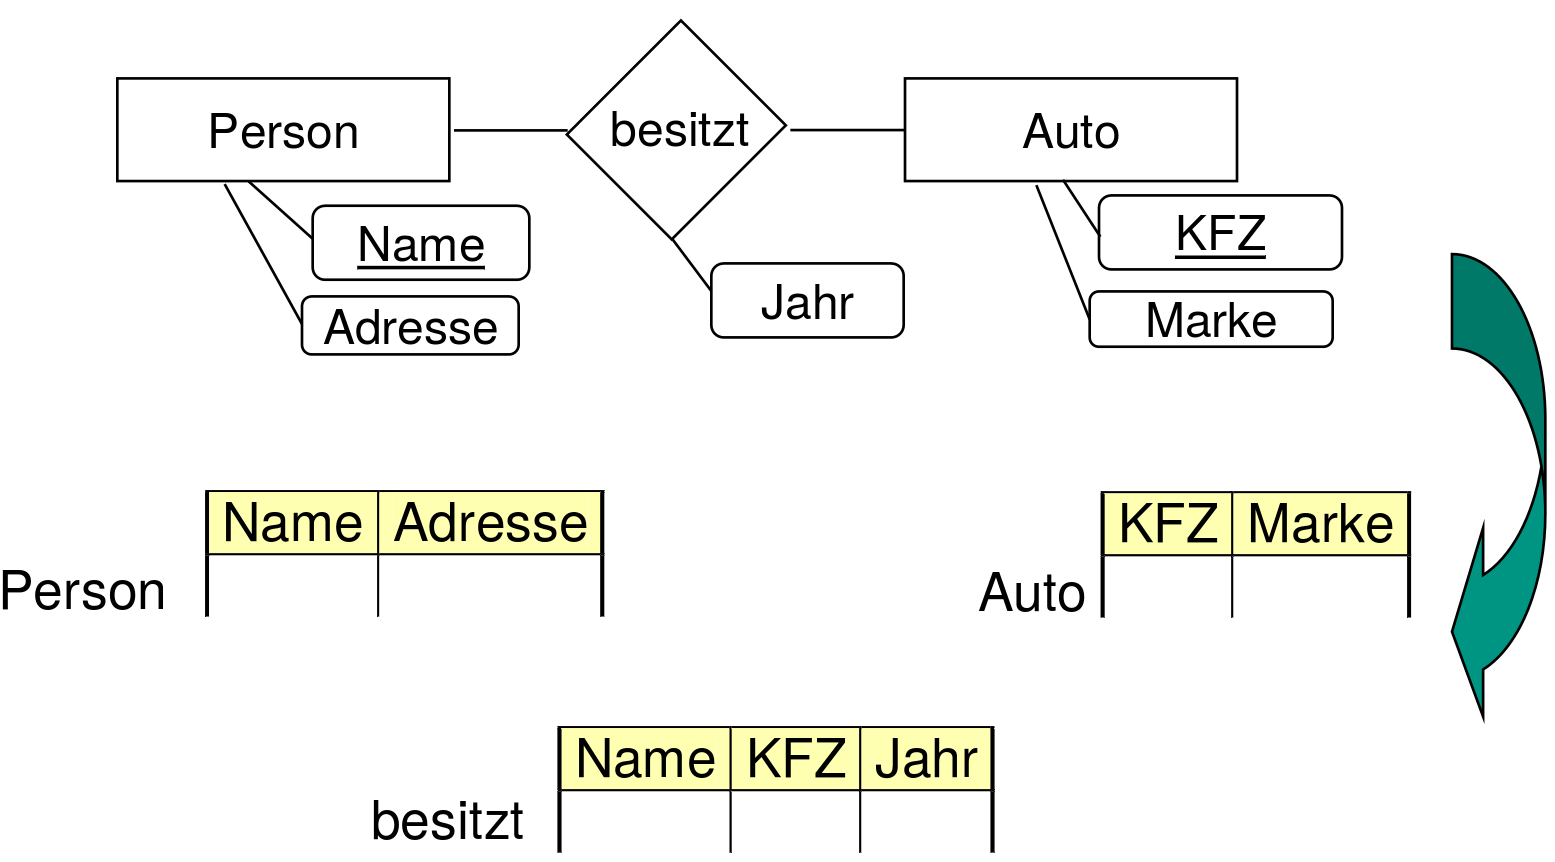
\includegraphics[width=.5\linewidth]{Abbilden}\end{figure}

\paragraph{Abbildungsziel: Kapazitätserhaltende Abbildung}
\begin{itemize}
	\item In beiden Fällen gleich viele Instanzen darstellbar
	\item \textbf{Zu Vermeiden:}
	\item Kapazitätserhöhend: relational mehr darstellbar als mit ER
	\item Kapazitätsvermindernd: relational weniger darstellbar als mit ER
\end{itemize}

\paragraph{Abbildungsregeln}
\begin{itemize}
	\item Entity-/Beziehungstypen \( \leadsto \) Relationenschemata \\* Attribute \( \leadsto \) Attribute Relationenschema \\* Schlüssel \( \leadsto \) übernehmen
	\item Kardinalitäten \( \leadsto \) Schlüsselwahl
	\item Ggf. Relationenschemata und Entity-/Beziehungstypen verschmelzen
	\item Einführung neuer Fremdschlüsselbedingungen: \\*
		- Teil der Schema-Definition \\*
		- Entstehen bei Abbildung von Relationships \\*
		- Ersetzen Linie von Relationship zu Entity
	\item Beziehungstyp \( \leadsto \) Relationenschema mit Attributen des Beziehungstyps und Primärschlüssel der beteiligten Entity-Typen
\end{itemize}
\begin{figure}[H]\centering\label{Abbilden2}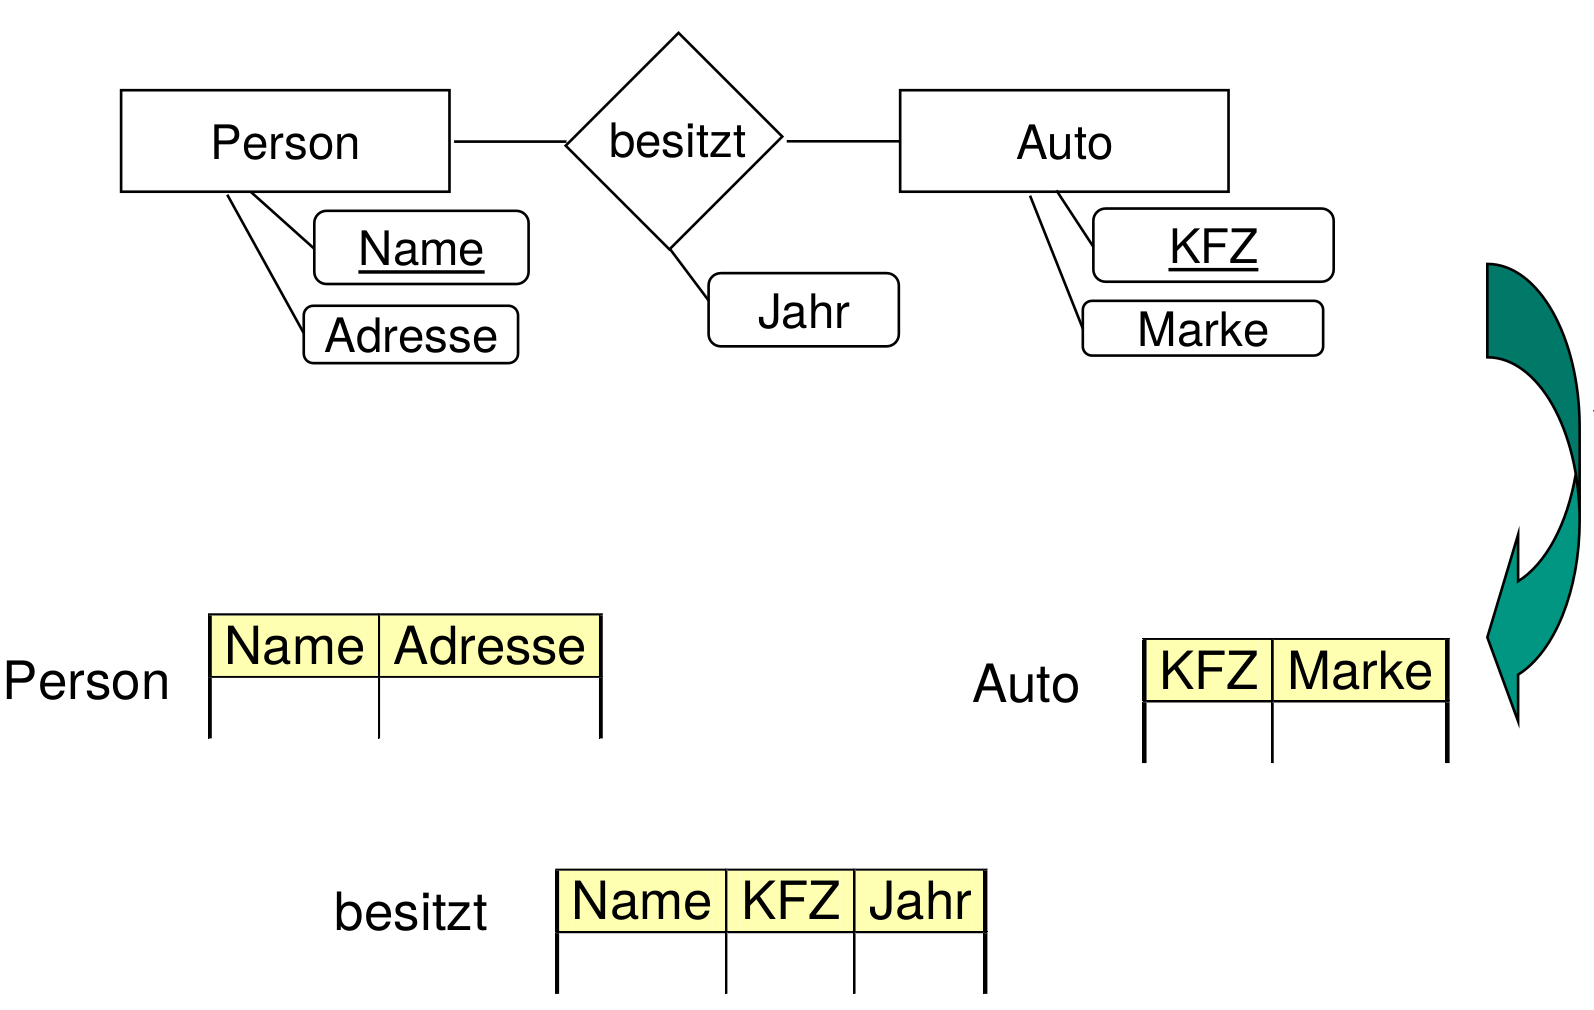
\includegraphics[width=.5\linewidth]{Abbilden2}\end{figure}

\begin{fragen}
	\item Warum gibt es im ER-Modell keine Fremdschlüssel?
	\item Was bedeutet ``kapazitätserhaltende Abbildung''? Geben Sie Beispiele.
	\item Wiedergabe der unterschiedlichen Beziehungsabbildungen (1:1, 1:n, m:n)
	\item In welchen Fällen lässt sich das Schema optimieren? Was bedeutet Optimierung hier?
	\item Wie lassen sich mengenwertige Attribute abbilden?
	\item Warum ist Abbildung der folgenden Konstrukte vom ER-Modell ins Relationenmodell problematisch? Rekursive Beziehungen, Partitionierung, Generalis.
\end{fragen}
  \section{Relationaler Datenbankentwurf}
\label{sec:abbildenRelational}

\paragraph{Funktionale Abhängigkeiten (FD)}
\begin{itemize}
	\item In Relation \( R(X,Y) \) ist \( Y \) von \( X \) funktional abhängig (schreibe \( X \to Y \)), falls zu jedem \( X \)-Wert genau ein \( Y \)-Wert gehört \\*
	 (z.B. ISBN $\to$ Buchtitel, Inventarnr. oder Stadt $\to$ Bundesland)
	\item \( \leadsto \) ``\( X \) bestimmt \( Y \)''
	\item Festlegung der FDs a priori beim Schemaentwurf (enthält semantische Information für höhere Konsistenz), nicht hinterher aus dem Datenbestand
	\item Spezialfall \textbf{Schlüssel} X für Relation R: $X \to R$ und X minimal
	\item \textbf{Transitiv}: $X \to  Y  \to  Z \Rightarrow  X  \to Z$
	\item \( F \): Menge von FDs (\emph{functional dependencies}), \( f \in F \) einzelne FD
	\item \( F \) impliziert \( f \): \( F \models f \)   $\qquad$  (bedeutet $SAT_R(F) \subseteq SAT_R(f)$)
	\item \textbf{Hülle}: \( F_R^+ = \{ f \mid (f \text{ FD über} R) \wedge F \models f \} \)
	\item Hülle einer Attributmenge X bezüglich F ist \\*
	$X^*_F := \{ A \mid X \to A \in F^+ \}$
	\item \textbf{Reflexiv}: $X \to X$ (und $F \models X \to X$ für alle F, X)
	\item \textbf{Akkumulativ}: $X \to YZ, Z \to VW \Rightarrow X \to YZV$
	\item \textbf{Projektiv}: $X \to YZ \Rightarrow X \to Y$
	\item Äquivalente FD-Mengen (Überdeckungen): \( F \equiv G \) falls \( F^+ = G^+ \)
\end{itemize}

\paragraph{RAP-Algorithmus für das Membership-Problem}
\begin{itemize}
	\item  Problem: Menge von FDs $F$. Gilt $X \to Y \in F^+$?
	\item Lösung in linearer Zeit: \\*
		1. $X^* :=  X$ (R-Regel) \\*
		2. Erweitere $X^* := X^* \cup Y_1$ für $X_1 \to Y_1$ mit $X_1 \subseteq X^*$ bis $X^*$ stabil (A-Regel) \\*
		3. Ist $Y \subseteq X^*$, gilt $X \to Y$ (P-Regel)
\end{itemize}

\paragraph{Redundanzen --- Anomalien}
\begin{itemize}
	\item Belegen unnötigen Speicherplatz
	\item Widersprüchliche oder fehlende Eingaben (\textbf{Einfügeanomalie})
	\item Änderungen parallel in allen Vorkommen nötig (\textbf{Updateanomalie})
	\item Informationen können beim Löschen anderer Inhalte mit verloren gehen (\textbf{Löschanomalie})
\end{itemize}

\paragraph{Abhängigkeitstreue}
\begin{itemize}
	\item Alle gegebenen Abhängigkeiten sind durch Schlüssel repräsentiert
	\item Genauer: Menge der Abhängigkeiten (FDs) äquivalent zur Menge der Schlüsselabhängigkeiten.
\end{itemize}

\paragraph{Verbundtreue}
\begin{itemize}
	\item Originalrelationen können durch Verbund der Basisrelationen wiedergewonnen werden
	\item Kriterium für zwei Relationen:
	Dekomposition von X in $X_1$ und $X_2$ verbundtreu, wenn $X_1 \cap X_2 \to X_1$ oder $X_1 \cap X_2 \to X_2$
	\item Allgemeines Kriterium: 
	Wenn eine abhängigkeitstreue Dekomposition von R in $X_i$ einen Universalschlüssel erhält (also für ein $X_i$ gilt $X_i \to R$), so ist sie verbundtreu.
\end{itemize}

\paragraph{Universalrelation}
\begin{itemize}
	\item \textbf{Universalrelation} (von \( R_1, \dots, R_n \)): \( R = R_1 \bowtie \cdots \bowtie R_n \)
	\item \textbf{Universalschlüssel}: Schlüssel der Universalrelation
	\item Beispiel: \( R_1, R_2, R_3 \):
	\begin{figure}[H]\centering\label{NonJoin}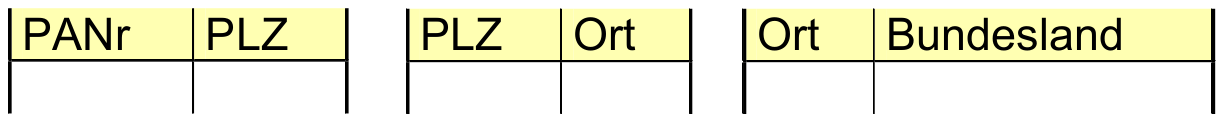
\includegraphics[width=.5\linewidth]{NonJoin}\end{figure}
	\item \quad \( R_1 \bowtie R_2 \bowtie R_3 \):
	\begin{figure}[H]\centering\label{Join}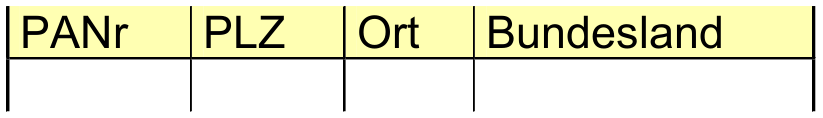
\includegraphics[width=.4\linewidth]{Join}\end{figure}
\end{itemize}



\paragraph{Entwurfsziel}
\begin{itemize}
	\item Relationenschemata, (Fremd-)Schlüssel so wählen, dass \\*
		- alle Anwendungsdaten aus Basisrelation hergeleitet werden können (\emph{Verbundtruee}) \\*
		- nur semantisch sinnvolle und konsistente Anwendungsdaten dargestellt werden können (\emph{Abhängigkeitstreue}) \\*
		- möglichst nicht-redundante Daten
\end{itemize}

\paragraph{Erste Normalform}
\begin{itemize}
	\item Nur \emph{atomare Attribute} in Relationenschemata
\end{itemize}

\paragraph{Zweite Normalform}
\begin{itemize}
	\item Keine \emph{partiellen Abhängigkeiten} eines Nicht-Primattributs von einem möglichen Schlüssel
	\item Auflösen durch Abtrennen der rechten und Kopie der linken Seite
	\item \textbf{Partielle FD}: Nicht-Primattribut hängt voll funktional von \textbf{einem Teil} eines Schlüsselkandidaten ab.
	\item \textbf{Volle FD}: \( \beta \) ist voll funktional abhängig von \( \alpha \), wenn aus \( \alpha \) kein Attribut entfernt werden kann, so dass FD immer noch gilt.
	\item Gegenbeispiel: PLZ, Bundesland \( \to \) Ort
\end{itemize}

\paragraph{Dritte Normalform}
\begin{itemize}
	\item Keine \emph{transitiven Abhängigkeiten} eines Nicht-Primattributs von einem möglichen Schlüssel
	\item \textbf{Transitive Abhängigkeit}: Schlüssel \( K \) bestimmt Attributmenge \( X \) funktional, diese wiederum bestimmt Attributmenge \( Y \) \\* 
	(und $X \nrightarrow K, \quad Y \notin KX$ ) \\*
	\( \leadsto \) Transitive Abhängigkeit \(K  \to X \to Y \)
	\item Erreichen durch Abspalten von \( Y \) und Kopie von \( X \)
	\item 3NF impliziert 2NF, da partielle Abhängigkeit Spezialfall von transitiver Abhängigkeit (wähle $X \subsetneq K$)
\end{itemize}

\paragraph{Boyce-Codd-Normalform}
\begin{itemize}
	\item Relationenschema \( \mathcal{R} \) mit FDs \( F \) ist in BCNF, wenn für jede FD \( \alpha \to \beta \) eine der folgenden Bedingungen gilt: \\*
		- \( \beta \subseteq \alpha \) (triviale Abhängigkeit) \\*
		- \( \alpha \) Schlüssel von \( \mathcal{R} \) (oder Obermege eines Schlüssels von \( \mathcal{R} \))
	\item Zerlegung von \( \mathcal{R} \) in \( \mathcal{R}_{1} = (\alpha \cup \beta), \mathcal{R}_{2} = \mathcal{R}-\beta \) \\* (\( F \ni f : \alpha \to \beta, \beta \) maximal)
	\item Verbundtreu: $R_1 \cap R_2 = \alpha$ ist Schlüssel von $R_1$
	\item Aber nicht immer Abhängigkeitstreu: Abhängigkeiten können beim Zerlegen verloren gehen!
	\item Dritte Normalform daher meist ausreichend
\end{itemize}

\paragraph{Minimalität}
\begin{itemize}
	\item Kriterien mit möglichst wenigen Relationenschemata erreichen
\end{itemize}

\paragraph{Dekomposition}
\begin{itemize}
	\item Prinzip: Immer wenn \( X \to Y \to Z \) wird Relation zerlegt
	\item Erreicht nur 3NF und Verbundtreue
	\item \textbf{Normalisierung}: Falls \( K \to X \to Y \), dann \( Y \) aus \( R \) entfernen und mit \( X \) in neues Relationenschema stecken
	\item Beispiel: \( U = \{ \text{PANr}, \text{PLZ}, \text{Ort}, \text{Land}, \text{Staat} \} \), \\*
	\( F = \{ \text{PANr} \to \text{PLZ}, \text{PLZ} \to \text{Ort}, \text{Ort} \to \text{Land}, \text{Land} \to \text{Staat} \} \) \\*
	\( \leadsto \) \( (U,K(F)) = (\{ \text{PANr}, \text{PLZ}, \text{Ort}, \text{Land}, \text{Staat} \}, \{ \{ \text{PANr} \} \}) \) \\*
	Betrachte \( \text{PANr} \to \text{Land} \to \text{Staat} \). Neue Relationen: \\*
		- \( R_1 = \{ \text{Land}, \text{Staat} \} \) \\*
		- \( R_2 = \{ \text{PANr}, \text{PLZ}, \text{Ort}, \text{Land} \} \)
	Wiederholen mit \( R_2 \)
	\item \textbf{Probleme}: Keine Abhängigkeitstreue, keine Minimalität, reihenfolgeabhängig, NP-vollständig (Schlüsselsuche)
\end{itemize}



\paragraph{Syntheseverfahren}
\begin{itemize}
	\item Prinzip: Synthese formt Original-FD-Menge \( F \) in Menge von Schlüsselabhängigkeiten \( G \) so um, dass \( F \equiv G \)
	\item Abhängigkeitstreue per Definition; Verbundtreue (nur mit Trick), 3NF und Minimalität werden reihenfolgeunabhängig erreicht
	\item Polynomielle Zeitkomplexität
	\item \emph{Verfahren}: \\*
		1. Redundanzen eliminieren: Entfernen überflüssiger FDs und Attribute	(\( f \) überflüssig wenn \( F \equiv F - \{  f \} \)) \\*
		2. FDs zu Äquivalenzklassen zusammenfassen: FDs in selber Klasse, wenn sie äquivalente linke Seiten haben \( \leadsto \) ein Relationenschema pro Äquivalenzklasse
	\item Beispiel: \( F = \{ A \to B, AB \to C, A \to C, B \to A, C \to E \} \) \\*
		1. Redundante FDs: \( A \to C \) (Stand: \( F' = \{ A \to B, AB \to C, B \to A, C \to E \} \)) \\*
		2. Überflüssige Attribute: \( B \) in \( AB \to C \) (Stand: \( F'' = \{ \underbrace{A \to B, A \to C, B \to A}_{\text{Äquivalenzklasse}}, C \to E \} \)) \\*
		3. Ergebnis Relationenschema: \( (ABC, \{ \{ A \}, \{ B \} \}), (CE, \{ \{ C \} \}) \)
	\item Trick \emph{Verbundtreue}: Orignal FD-Menge um $R \to \delta$ erweitern
\end{itemize}

\paragraph{Mehrwertige Abhängigkeiten}
\begin{itemize}
	\item \textbf{Mehrwertige Abhängigkeit} (\emph{multi value dependency, MVD}): \\*
		Jeder Wert des abhängigen Attributes kommt in Kombination mit allen Werten der anderen Attribute vor
	\item Redundanzbehaftet
	\item Beispiel:
	\begin{center}
		\begin{tabular}{|lll|}
		  \hline
		  \emph{Kurs} & \emph{Buch} & \emph{Dozent} \\
		  \hline
		  AHA & Silberschatz & John D \\
		  AHA & Nederpelt & John D \\
		  AHA & Silberschatz & William M \\
		  AHA & Nederpelt & William M \\
		  \hline
		\end{tabular}
	\end{center}
	Neues Buch: für jeden Dozenten anlegen \( \leadsto \) MVD
\end{itemize}

\paragraph{Vierte Normalform}
\begin{itemize}
	\item Beispiel: Relation mit Attributen \emph{Name}, \emph{Neffe}, \emph{Hobby} \\*
		Es gelte MVD: \emph{Name} \( \twoheadrightarrow \) Neffe \\*
		Wenn (Heinrich, Martin, Autos) und (Heinrich, Thomas, Basteln) 
		\( \in r \), dann auch 
		(Heinrich, Martin, Basteln) und (Heinrich, Thomas, Autos)
	\item Formal: \( r \) genügt MVD \( X \twoheadrightarrow Y \Leftrightarrow \) \\*
		\( \forall t_1, t_2 \in r: [(t_1 \neq t_2 \wedge t_1(X) = t_2(X)) \\* \Rightarrow \exists t_3 \in r: t_3(X)=t_1(X) \wedge t_3(Y)=t_1(Y) \wedge t_3(Z) = t_2(Z) ] \) 
	\item 4NF: solche MVDs aufspalten
	\item Trivial, wenn keine weiteren Attribute im zugehörigen Schema
\end{itemize}

\begin{fragen}
	\item Erläutern Sie die folgenden Begriffe: Redundanz, Funktionale Abhängigkeit, Normalform, Verbundtreue, Abhängigkeitstreue, Minimalität.
	\item Erläutern Sie die Aussage: ``Funktionale Abhängigkeiten beinhalten semantische Informationen.''
	\item Welche Anomalien kennen Sie? Erläutern Sie für jede dieser Anomalien, warum Sie störend ist.
	\item Warum braucht man für Verbundtreue Kriterien, für Abhängigkeitstreue jedoch scheinbar nicht?
	\item Welche Normalformen kennen Sie? Sagen Sie umgangssprachlich, wie sie definiert sind.
\end{fragen}
  \section{Relationale Datenbanksprachen}
\label{sec:sql}

\paragraph{SQL-Kern}
\begin{items}
	\item \textbf{select} \\*
		Projektionsliste \\*
		Attribute, arithmetische Ausdrücke, Aggregatfunktionen \\*
		\emph{select distinct}: keine Dopplungen\\*
		Umbenennungen: \lstinline[language=sql]{select Preis * 1.44 as DollarPreis }
	\item \textbf{from} \\*
		Zu verwendende Relationen, Umbenennungen\\*
		Orthogonalität: Wiederum SFW-Block möglich\\*
		\lstinline[language=sql]{select * from (select [...]) where [...] }
	\item \textbf{where} \\*
		Selektions- und Verbundbedingungen, \\*
		geschachtelte Anfragen (wieder SFW-Block)
	\item \textbf{group by} \\*
		Gruppierung für Aggregatfunktionen
	\item \textbf{having} \\*
		Selektionsbedingungen an Gruppen
\end{items}

\paragraph{from --- Mehrere Relationen}
\begin{items}
	\item Bei mehr als einer Relation: \emph{Kartesisches Produkt}
	\item Kommagetrennt oder als expliziter Operator:
	\begin{lstlisting}[language=sql]
select * from Kuenstler K, Titel T
select * from Kuenstler cross join Titel
	\end{lstlisting}
\end{items}

\paragraph{Natürlicher Verbund}
\begin{items}
	\item Automatischer Equi-Join auf allen übereinstimmenden Spalten, diese erscheinen nur ein mal in der Ergebnisrelation
	\begin{lstlisting}[language=sql]
select * from Kuenstler natural join Titel
	\end{lstlisting}
\end{items}

\paragraph{Theta-Join}
\begin{items}
	\item Verbund über Verbundsbedingungen
	\begin{lstlisting}[language=sql]
select * from Kuenstler 
	join Titel on Kuenstler.KID = Titel.KID
	\end{lstlisting}
	\item Beispiel: \(  \text{Auto} \bowtie_{AutoPreis > BootPreis} \text{Boot} \)
\end{items}

\paragraph{Outer, Left, Right Join}
\begin{items}
	\item Dangling Tuples übernehmen und mit Nullwerten füllen
	\begin{figure}[H]\centering\label{SQLJoin}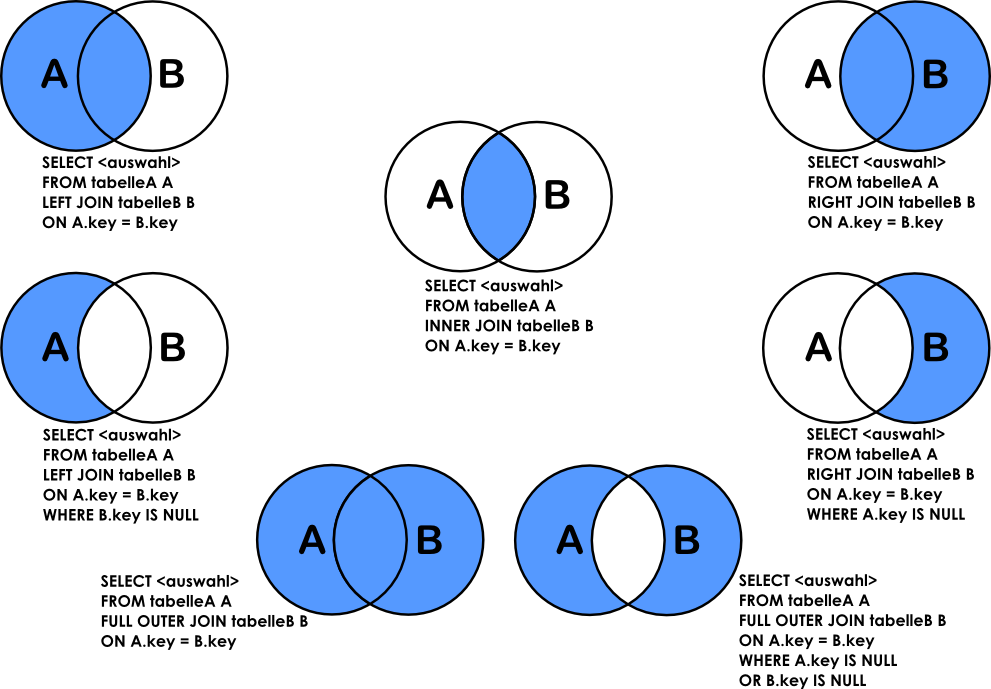
\includegraphics[width=0.4\textwidth]{SQLJoin}\end{figure}
\end{items}

\paragraph{Self-Join}
\begin{items}
	\item Kartesisches Produkt einer Tabelle mit selbst
	\begin{lstlisting}[language=sql] 
	select * from SNUser eins, SNUser zwei
	where eins.Alter < zwei.Alter
	\end{lstlisting}
	Vierspaltiges Ergebnis:
	\begin{lstlisting}[language=sql]
eins.Name, eins.Vorname, zwei.Name, zwei.Vorname
	\end{lstlisting}
	\item Anwendungen: Vergleichen oder Zählen von Wertemengen
\end{items}



\paragraph{where}
\begin{items}
	\item Konstanten-Selektion: \\*
	\lstinline[language=sql]{select * from Buecher where Buecher.Titel = "Titel"}
	\item Verbundbedingung bei Cross-Join (Attribut-Selektion):
	\begin{lstlisting}[language=sql]
select Buecher.Titel, Buecher_Stichwort.Stichwort
	from Buecher, Buecher_Stichwort
	where Buecher.ISBN = Buecher_Stichwort.ISBN
	\end{lstlisting}
	\item \lstinline[language=sql]{like}: Ungewissheitsselektion
	(\lstinline[language=sql]{where name like "C\%"})\\*
	'\%' --- Beliebig viele Zeichen $\qquad$ '\_' --- Genau ein Zeichen
	\item \lstinline[language=sql]{and, or, not, is null}
	\item \lstinline[language=sql]{in}: \lstinline[language=sql]{where ISBN in (select ISBN from Empfiehlt)}
\end{items}

\paragraph{Verzahnt geschachtelte Anfragen}
\begin{items}
	\item In der inneren Anfrage Attribute aus der äußeren verwenden
	\begin{lstlisting}[language=sql]
select Nachname from Personen
where 1.0 in (select Note from Prueft
	where PANr = Personen.PANr)
	\end{lstlisting}
	\item \lstinline[language=sql]{Exists}: Test, ob Ergebnis der inneren Anfrage nicht leer ist
	\begin{lstlisting}[language=sql]
select ISBN from Buch
where exists (select * from Ausleihe
	where Invnr = Buch.Invnr)
	\end{lstlisting}
\end{items}

\paragraph{Mengenoperationen}
\begin{items}
	\item Übernimmt Attributnamen des linken Operanden
	\item Vereinigung
	\begin{lstlisting}[language=sql]
select A, B, C from R1 union [all]
	select A, C, D from R2
	\end{lstlisting}
	\item \lstinline[language=sql]{union all}: Duplikate werden behalten
	\item Differenz: \lstinline[language=sql]{except}
	\item Durchschnitt: \lstinline[language=sql]{intersect}
\end{items}

\paragraph{Aggregatfunktionen}
\begin{items}
	\item Prinzip: Berechnung eines Werts aus Werten eines Attributs\\*
		\lstinline[language=sql]{ sum([all / distinct] Attributname) }
	\item Standard SQL: \lstinline[language=sql]{count(), sum(), min(), max(), avg()}
	\item Speziell: \lstinline[language=sql]{count(*)}
	\item Modifikatoren: \lstinline[language=sql]{all / distinct} (Voreinstellung: all)
\end{items}

\paragraph{Group by}
\begin{items}
	\item Gruppierung G: Für gleiche G-Werte werden Resttupel in Relation gesammelt, darauf dann Aggregatfunktionen angewendet
	\item
	\begin{lstlisting}[language=sql]
select Marke, sum(Anzahl)
	from Zulassungen
	group by Marke
	\end{lstlisting}
	\item \emph{Wichtig:} Jedes Select-Attribut muss entweder Gruppiert oder Aggregiert werden!
	\item \lstinline[language=sql]{having}: Bedingung auf gruppierter Relation
	\begin{lstlisting}[language=sql]
select PANr, sum(Entlohnung)
	from anstellungen
	group by PANr
	having sum(entlohnung) > 10000
	\end{lstlisting}
	
	\item
	\begin{lstlisting}[language=sql]
select Matrikelnr from Pruefung
	group by Matrikelnr
	having avg(Note) < (select avg(Note) from Pruefung)
	\end{lstlisting}
\end{items}



\paragraph{Quantoren}
\begin{items}
	\item \lstinline[language=sql]{any/some} (äquivalent):
	\begin{lstlisting}[language=sql]
select PANr, ImmaDatum
	from Studenten
	where MatNr = any (select MatNr from Prueft)
	\end{lstlisting}
	\item \lstinline[language=sql]{all}:
	\begin{lstlisting}[language=sql]
select Name from Kunde, Bestellung
	where Kunde.id = Bestellung.KundeID
	and bestellwert > ALL (SELECT avg(bestellwert) 
		from Bestellung group by KundeID)
	\end{lstlisting}
	\item Aber: Anwendbarkeit eingeschränkt, z.B. kein Vergleich auf Mengengleichheit
\end{items}

\paragraph{order by}
\begin{items}
	\item Menge von Tupeln $\leadsto$ Sortierte Liste
	\begin{lstlisting}[language=sql]
select MatNr, Note from Prueft
	where V_Bez = 'DBS'
	order by Note [asc / desc], MatNr
	\end{lstlisting}
	\item Aufsteigend (\lstinline[language=sql]{asc}, Standard) oder Absteigend (\lstinline[language=sql]{desc})
	\item \emph{Wichtig}: Sortier-Attribut(e) müssen in Select vorkommen!\\*
	Denn: Sortierung wird auf das Ergebnis der vorherigen SFW-Anfrage angewendet.
\end{items}

\paragraph{Nullwerte}
\begin{items}
	\item Vergleiche mit Nullwert: \lstinline[language=sql]{unknown} statt \lstinline[language=sql]{true} oder \lstinline[language=sql]{false} \\*
	\( \leadsto A=A \) keine Tautologie!
	\item Deshalb \emph{nicht gleich}: \lstinline[language=sql]{select * from Person} und \\* \lstinline[language=sql]{select * from Person where Name = Name}\\*
	(Letzteres eliminiert Tupel mit Name = null)
\end{items}

\paragraph{Änderungsoperationen}
\begin{items}
	\item \emph{Insert}
	\begin{lstlisting}[language=sql]
insert into relation [(attribut1, ...)]
	values (wert1, ...)
	\end{lstlisting}
	
	\item Auch SQL-Anfragen als Wert möglich.
	\begin{lstlisting}[language=sql]
insert into Kunde (select LName, LAdr, 0 from Lieferant)
	\end{lstlisting}
	
	\item \emph{Update}
	\begin{lstlisting}[language=sql]
update relation set attribut1 = wert, ... 
	[where bedingung]
	\end{lstlisting}
	
	\item \emph{Delete}
	\begin{lstlisting}[language=sql]
delete from relation [where bedingung]
	\end{lstlisting}
\end{items}

\begin{fragen}
	\item Formulieren diverser (komplexer) SQL-Anfragen
	\item Vorgegebene geschachtelte Anfrage als nicht-geschachtelte schreiben
	\item Welche Join-Varianten kennen Sie?
	\item Geben Sie ein Beispiel an, in dem ein Self-Join sinnvoll ist.
	\item Was ist der Zusammenhang zwischen Vereinigung und Outer Join?
	\item Was ist eine Umbenennung im SQL-Kontext? Wann wird sie gebraucht?
	\item Geben Sie ein sinnvolles Beispiel für eine Anfrage an, die eine having-Klausel hat.
	\item Geben Sie ein Bespiel für eine Anfrage mit einer having-Klausel an, bei der man \\*
		- die Klausel durch eine where-Klausel ersetzen kann, \\*
		- das nicht kann.
	\item Erläutern Sie, warum im SQL-Kontext ``A==A'' keine Tautologie ist.
\end{fragen}
  \section{Nebenläufigkeit, Transaktionen}
\label{sec:parallel}

\paragraph{Transaktion}
\begin{items}
	\item Partiell geordnete Folge von Lese- und Schreibzugriffen auf Datenobjekte (mit Commit oder Abort am Ende)
	\item \textbf{ACID Eigenschaften:}
	\item Atomicity: Entweder alles oder gar nichts ausführen
	\item Consistency: Integritätsbedingungen bleiben erhalten
	\item Isolation: Nutzer hat Eindruck, er wäre alleine
	\item Durability: Änderungen sollen dauerhaft sein
\end{items}

\paragraph{Synchronisation}
\begin{items}
	\item Viele Nutzer sollen Daten gleichzeitig lesen und schreiben können
		\\*
		\( \leadsto \) Konsistenz sicherstellen \( \leadsto \) \emph{Synchronisationskomponente}
	\item \textbf{Serielle Ausführung}: 
		\\*
		+ Konsistenz immer gewährleistet 
		\\*
		$-$ extreme Wartezeiten, schlechte Ressourcenausnutzung
\end{items}

\paragraph{Unkontrollierte nicht-serielle Ausführung: Probleme}
\begin{items}
	\item \emph{Lost Update}\\
		 Programm \( T_1 \) transferiert 300 EUR von Konto \( A \) nach \( B \),
		\\*
		Programm \( T_2 \) schreibt Konto \( A \) \( 3 \% \) Zinsen gut
		\\*
		\( \leadsto \) Zinsen aus \( S_5 \) von \( T_2 \) verloren, weil \( T_1 \) in \( S_6 \) überschreibt

	\begin{figure}[H]\centering\label{Synchronisation}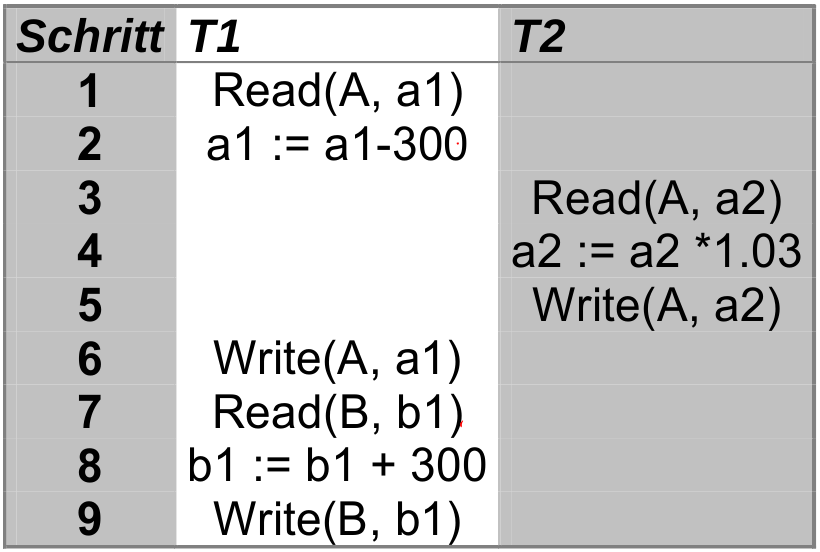
\includegraphics[width=0.2\textwidth]{Synchronisation}\end{figure}
	
	\item \emph{Dirty Read}\\
		Commit, Abort \\
		\( T_2 \) schreibt Zinsen gut basierend auf einem Wert, der nicht zu einem konsistenten Zustand gehört, denn später erfolgt Abort von \( T_1 \)

	\begin{figure}[H]\centering\label{DirtyRead}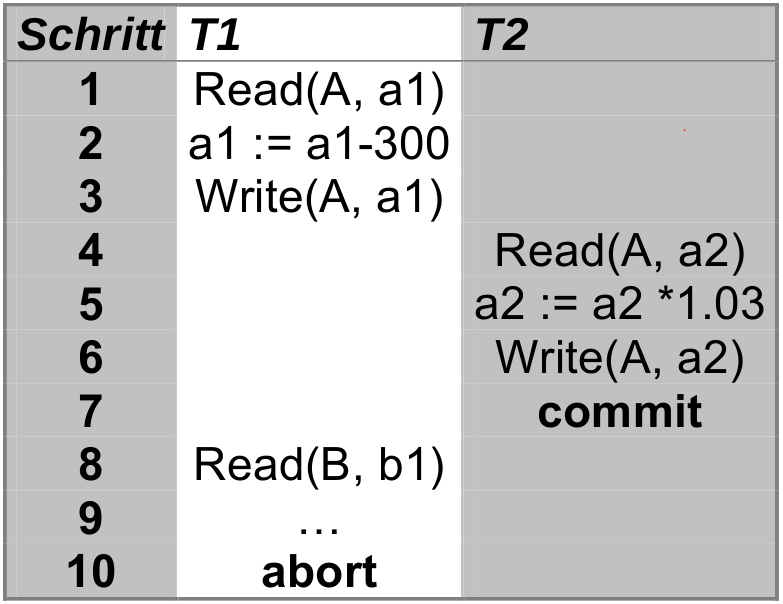
\includegraphics[width=0.2\textwidth]{DirtyRead}\end{figure}
	
	\item \emph{Non-Repeatable Reads}\\
		 Programm liest Datenobjekt mehr als einmal und sieht dabei Änderung durch anderes Programm
	\begin{figure}[H]\centering\label{NonRepeatableRead}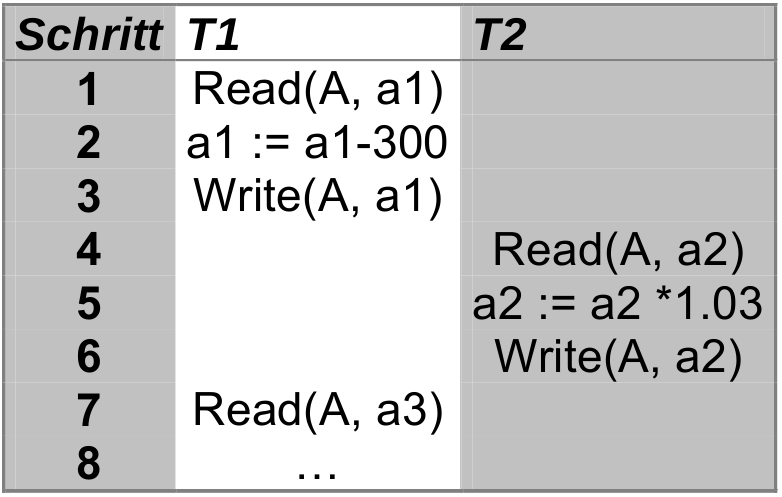
\includegraphics[width=0.2\textwidth]{NonRepeatableRead}\end{figure}
	
	\item \emph{Phantom}\\
		Berechnung von Änderung auf veralteten Werten
\end{items}

\paragraph{Konflikt}
\begin{items}
	\item Zwei Operationen \( p, q \) konfligieren
		\\*
		\( \Leftrightarrow \) \( p,q \) greifen auf selbes Datenobjekt zu und \( p \) oder \( q \) ist Schreiboperation
	\item In einer Transaktion müssen konfligierende Operationen \emph{geordnet sein} (andere nicht zwingend)
\end{items}

\paragraph{Histories}
\begin{items}
	\item \textbf{Vollständige Historie}: Menge von Transaktionen und Ausführungsordnung (nebenläufige Verzahnung, Ordnung konfligierender Operationen zwischen Transaktionen)
	\item \textbf{Historie}: Präfix einer vollständigen Historie
	\item \textbf{Commited Projection} (\( C(H) \)): H nach Entfernen aller nicht-committeten Operationen
	\item Eine Eigenschaft von Histories ist \emph{prefix commit closed}
		\\*
		\( \Leftrightarrow \) (\( H \) erfüllt Eigenschaft \( \Rightarrow C(H') \) erfüllt Eigenschaft)
\end{items}

\paragraph{Konfliktäquivalenz (CSR)}
\begin{items}
	\item \( H, H' \) (Konflikt-)Äquivalent, wenn \\*
		- gleiche Transaktionen, gleiche Operationen \\*
		- gleiche Ordnung konfligierender Operationen (gleiche Konfliktrelation)
\end{items}

\paragraph{Serialisierbarkeit}
\begin{items}
	\item \( H \) serialisierbar \( \Leftrightarrow C(H) \equiv H_S \) (serielle History)
	\item \textbf{Serialisierbarkeitsgraph} (Abhängigkeitsgraph):
		\\*
		Knoten = Transaktionen
		\\*
		(gerichtete) Kante von $T_1$ nach $T_2$ wenn $op_1$ und $op_2$ konfligieren und $op_1 < op_2$
	\item \emph{Theorem}: Schedule ist serialisierbar, wenn entsprechender Abhängigkeitsgraph zykelfrei ist
	\item Konflikt-Serialisierbarkeit ist prefix commit-closed
	\item \emph{Ansatz nicht praktikabel}: \\*
		- Serialisierbarkeit nur im Nachhinein überprüfbar \\*
		- Administrativer Overhead zu hoch: Abhängigkeiten zu bereits terminierten Transaktionen berücksichtigen
\end{items}

\paragraph{Rücksetzbarkeitsklassen}
\begin{items}
	\item \textbf{Rücksetzbar (RC)}: Commit für $T_j$ erst erlaubt, wenn alle $T_i$ von denen $T_j$ liest, committed sind (Abort darf Semantik von bereits committeten Transaktionen nicht verändern).
	\item \textbf{Avoid cascading aborts (ACA)}: Nur Objekte von bereits committeten Transaktionen lesen.
	\item \textbf{Striktheit (ST)}: Objekte von noch nicht committeten Transaktionen dürfen weder gelesen noch überschrieben werden (ermöglicht einfache Implementierung des Rücksetzens)
\end{items}

\paragraph{Locking}
\begin{items}
	\item Lock für jedes Datenobjekt und jede Operationsart
		\\*
		Notation: \( rl_i[x] \), \( wl_i[x] \)
	\item Aber: Sperrdisziplin alleine reicht für Korrektheit nicht aus!
	
	\item \emph{Zwei-Phasen-Sperrprotokoll (2PL)}: \\*
		1. Locks werden hinzugenommen \\*
		2. Locks werden freigegeben
	\( \leadsto \) Serialisierbarkeit sichergestellt\\
						Deadlocks sowie kaskadierende Abbrüche weiterhin möglich
	
	\item \emph{Strenges Zwei-Phasen-Sperrprotokoll (S2PL)}: 
	
	Atomare Freigabephase am Ende der Transaktion\\
	\( \leadsto \) Zusätzlich ACA: Vermeidung kaskadierender Abbrüche
	
	\item \emph{Konservatives Zwei-Phasen-Sperrprotokoll (C2PL)}:
	
	Atomare Anforderungsphase zu Beginn der Transaktion\\
	\( \leadsto \) Zusätzlich: Vermeidet Deadlocks
	
	\item \emph{CS2PL}: 
	
	Kombination aus streng und konservativ: Atomare Anforderungs- und atomare Freigabephase \\
	\( \leadsto \) Serialisierbarkeit, ACA, Deadlockfreiheit
	
	\item \emph{Aber:} Jede Einschränkung schränkt auch die Zahl der möglichen Histories ein und verringert damit den möglichen Grad der Parallelität!
	
\end{items}

\begin{fragen}
	\item Was ist Isolation? Was ist der Zusammenhang zwischen Isolation und Serialisierbarkeit?
	\item Welche Probleme können bei unkontrollierter nebenläufiger Ausführung von Transaktionen auftreten?
	\item Beispiele für Lost Updates, Non-Repeatable Reads usw. angeben, die bestimmte Bedingungen erfüllen
	\item Warum ist es wichtig, dass unser Korrektheitskriterium für Histories prefix commit closed ist? Erklären Sie, warum Konflikt-Serialisierbarkeit prefix commit closed ist.
	\item Ist eine gegebene History serialisierbar/recoverable/cascadeless?
	\item Haben zwei Konflikt-äquivalente Histories stets die gleichen Reads-from-Beziehungen?
	\item Warum verwendet man in der Regel nicht den Serialisierbarkeitsgraphen, um Serialisierbarkeit sicherzustellen?
	\item Bei Deadlocks wird in der Regel eine Transaktion zurückgesetzt. Kann es vorkommen, dass die gleiche Transaktion mehrmals/beliebig oft zurückgesetzt wird? Wenn ja, was kann man jeweils dagegen tun?
	\item Geben Sie ein Beispiel für eine serialisierbare Ausführung, bestehend aus drei Transaktionen, mit folgender Eigenschaft an: Die zeitliche Reihenfolge der Commits ist \( c_1 \) vor \( c_2 \) vor \( c_3 \), die der äquivalenten seriellen Ausführung jedoch \( c_3 \) vor \( c_2 \) vor \( c_1 \).
	\item Um einen Deadlock aufzulösen muss eine der beteiligten Transaktionen zurückgesetzt werden. Welche Kriterien sind Ihres Erachtens nach sinnvoll, um diese Auswahl zu treffen?
\end{fragen}
  \section{Cloudsysteme --- Konsistenz}
\label{sec:cloudkonsistenz}

\paragraph{Verteilung}
\begin{items}
	\item \textbf{Vorteile} (scheinbar): \\*
		+ Leselastverteilung \\*
		+ Beschleunigung (durch höhere Lokalität) \\*
		+ Höhere Ausfallsicherheit
	\item \textbf{Nachteile}: \\*
		- Transaktionen müssen auf Knoten gleich angeordnet sein \\*
		- Widerspruchsfreie Anordnungsentscheidungen nötig für Konfliktfreiheit \( \leadsto \) schlechte Skalierbarkeit \\*
		- Für Konsistenz müssen alle Knoten verfügbar sein \( \leadsto \) geringere Ausfallsicherheit
	\item \( \leadsto \) Netzwerkpartitionierung
	\item \textbf{CAP-Theorem}: Wenn Netzwerkpartitionierung möglich, dann sind hohe Verfügbarkeit und Datenbestandskonsistenz unvereinbar
\end{items}

\paragraph{Eventual Consistency}
\begin{items}
	\item ``Wenn ab Zeitpunkt keine Änderungen mehr, dann werden irgendwann alle Lesezugriffe gleichen Wert zurückliefern''
	\item Alternativ: ``\dots dann werden irgendwann alle Lesezugriffe zuletzt geschriebenen Wert zurückliefern''
	\item Beispiel (social network): Netzwerkpartition
	\begin{items}
		\item Starke Konsistenz: Vorübergehend keine Postings möglich
		\item Eventual Consistency: User kann Posting schreiben, Follower sehen es sobald möglich
	\end{items}
\end{items}

\begin{fragen}
	\item Geben Sie die Probleme mit dem klassischen, starken Konsistenzbegriff im verteilten Fall wieder.
	\item Bekommt man mit \emph{eventual consitency} irgendeine Form von Sicherheit? Begründen Sie Ihre Antwort.
	\item Warum kann man im Bank-Kontext in manchen Situationen doch auf starke, klassische Konsistenz verzichten?
	\item Geben Sie ein weiteres Beispiel für eine Folge von Operationen, deren Anordnung egal ist.
\end{fragen}
  \section{Cloudsysteme --- Funktionalität}
\label{sec:cloudfunktionalitaet}

\paragraph{Was ändert sich in der Cloud?}
\begin{itemize}
	\item Physischer Entwurf muss automatisch erfolgen
	\item Obligatorische Datenverteilung
	\item Anfrageauswertung in Gegenwart anderer Anfragen
		\\*
		\( \leadsto \) entsprechende Planung
	\item Unterschiedliche QoS-Vereinbarungen mit unterschiedlichen Dienstnehmern
	\item Plötzliche extreme Zunahme von Zugriffen eines Dienstnehmers i.A. nicht vorhersehbar 
		\\*
		\( \leadsto \) Infrastruktur sollte damit umgehen können
	\item \emph{Secure Storage}: Verschlüsselung der Daten, trotzdem soll Dienstanbieter möglichst großen Teil der Anfrageauswertung übernehmen
\end{itemize}

\paragraph{Relationale Algebra}
\begin{itemize}
	\item \textbf{Projektion} $\pi$: Optimierung: bei vielen Projektionen hintereinander reicht die zuletzt ausgeführte auch allein:
		\\*
		\( \pi \)\lstinline{[KName](}\( \pi \)\lstinline{[KName, Land](Kuenstler))} \( \leadsto \) \( \pi \)\lstinline{[KName](Kuenstler)}
	\item \textbf{Selektion} $\sigma$: Optimierung: Selektionen lassen sich beliebig vertauschen, manchmal auch Projektion und Selektion
	\item \textbf{Verbund} $\bowtie$: Kommutativ, Assoziativ (Aber: Ausführungsreihenfolge kann erhebliche Performance-Unterschiede erzeugen)
		\\*
		\emph{Nested-Loop Join}: Teuer ($O(n * m)$), da pro Eintrag links über alle rechten Einträge iteriert wird. \\*
		Besser: \emph{Bock-Nested-Loop Join }(Arbeitsspeicher ausnutzen)
		\\*
		\emph{Merge Join}: Beide Relationen sortieren, dann Eintrag für Eintrag Merge-Technik anwenden (linear wenn X Schlüssel)
\end{itemize}

\paragraph{Logische vs. physische Operatoren}
\begin{itemize}
	\item DBS enthält meist mehrere pysische Operatoren und Implementierungen für den gleichen logsichen Operator
	\item DBS sucht selbst den optimalen pysischen Operator heraus
	\item Pysische Operatoren können dabei mehrere logische Operatoren zusammenfassen
\end{itemize}

\paragraph{Blockierende/Nichtblockierende Operatoren}
\begin{itemize}
	\item Operator blockiert \( \Leftrightarrow \) Ergebnis des Operators muss vor Ausführung des nachfolgenden vollständig berechnet sein \\* (z.B. Sort-Operator)
\end{itemize}

\paragraph{Histogramme}
\begin{itemize}
	\item Zeigt Auftrittshäufigkeit eines Intervalls (Bucket)
	\item \textbf{Equi-Width-Histogramm}: Breite aller Buckets gleich
	\item \textbf{Equi-Depth-Histogramm}: Auftrittshäufigkeit aller Buckets gleich
	\item Nützlich bei ein-Attribut-Anfragen, sonst nicht so:
		\\*
		Mehrdimensionale Histogramme schwer konstruierbar und wartbar, Anzahl Attributkombinationen exponentiell wachsend zur Anzahl der Attribute
\end{itemize}

\paragraph{Synchroner und asynchroner Zugriff}
\begin{itemize}
	\item \textbf{Synchron}: innerhalb einer Transaktion
	\item \textbf{Asynchron}: mehrere Transaktionen
\end{itemize}

\paragraph{Service-Level Agreements}
\begin{itemize}
	\item Vereinbarung zwischen Client und Server bzgl. Dienstausführung
		\\*
		``Antwort innserhalb von 300ms für 99,9\% der Aufrufe bei 500 Zugriffen pro Sekunde''
\end{itemize}

\paragraph{Quorum Consensus}
\begin{itemize}
	\item Szenario: Replikation mit \( n \) Knoten
		\\*
		\( \leadsto \) Wie strenge Konsistenz beim Schreiben sicherstellen? Was, wenn nicht alle Knoten verfügbar?
	\item Lesen: Lese Mindestanzahl von Versionen (\( R \)), nehme aktuelle
	\item Schreiben: Aktualisiere Mindestanzahl von Kopien (\( W \))
	\item Jede Kopie erhält Versionsnummer
	\item Üblich ist \( Q_R+Q_W > N \)
\end{itemize}



\paragraph{P2P}
\begin{itemize}
	\item \emph{peer to peer}-Systeme:
		\\*
		Jeder Knoten für Ausschnitt des Schlüsselraums verantwortlich
		\\*
		Verwaltung von (Schlüssel, Wert)-Paaren
		\\*
		(put, get)-Interface
		\\*
		Zu Größe des Schlüsselraums logarithmischer Suchaufwand
	\item Beispiel: \emph{Chord} \\*
		Zentrale Datenstruktur: \emph{identifier circle}, \emph{chord ring}\\*
		Schlüssel $k$ gehört zum im Uhrzeigersinn nächsten Knoten\\*
		Einfaches Hinzufügen / Entfernen von Knoten möglich
		\\* Suche: Jeder Knoten hat \emph{finger table}, \emph{i}-ter Eintrag von Knoten \( n \): successor(\( n+2^{i-1} \)) (\( m \) Anzahl Bits)
	\begin{figure}[H]\centering\label{Chord}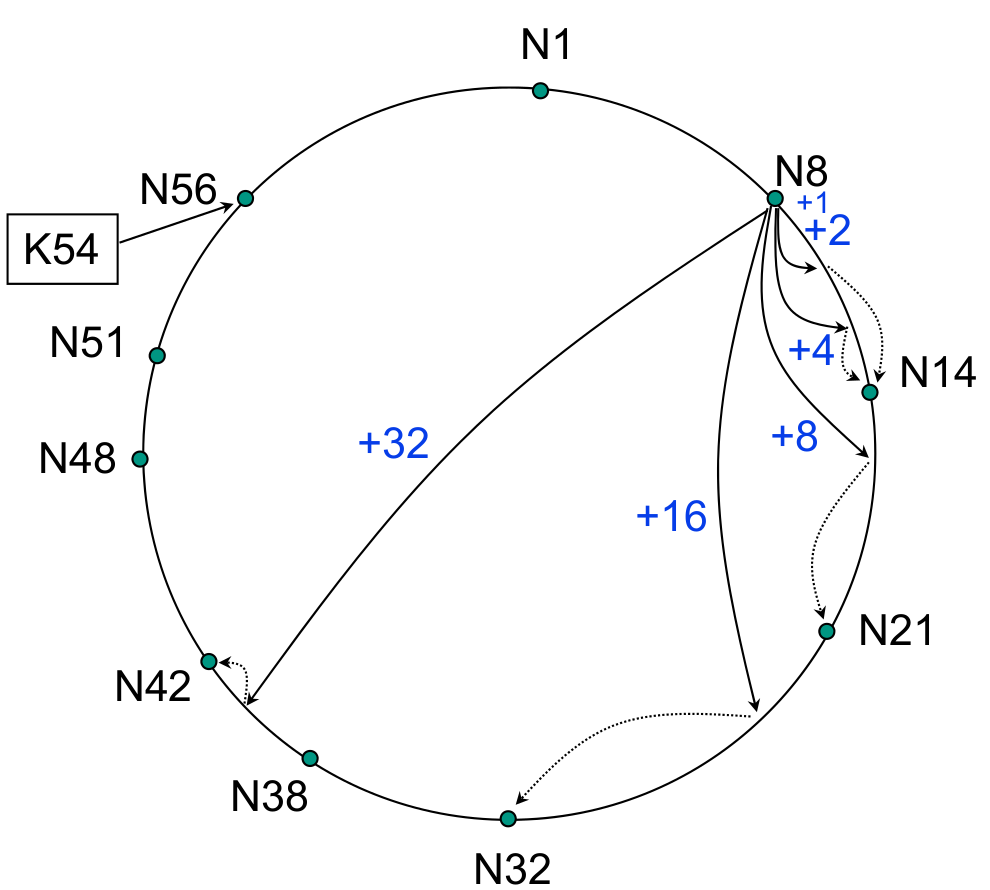
\includegraphics[width=.3\linewidth]{Chord}\end{figure}
	\item Replikation über \emph{chained replication}: Schlüssel nicht nur bei einem Knoten, sondern auch bei \( k \) Nachfolgern einfügen
	\item \textbf{Heterogenität}: Knoten können unterschiedlich leistungsstark sein (ggf. unterschiedliche Zuständigkeitsbereiche, unterschiedliche Last)
	\item Umrechnen von Anwendungs- in Systemschlüssel, um Last zu verteilen (gleich / ungleich, evtl. auf mehrere Positionen)
\end{itemize}

\paragraph{Dynamo}
\begin{itemize}
	\item Key-Value-Store
	\item get-/put-Interface
	\item Objekte BLOBs \( \leadsto \) kein DB-Schema \( \leadsto \) Interpretieren nötig
	\item Keine Isolation \( \leadsto \) keine totale Konsistenz
	\item Schreibzugriff jeweils nur für ein Objekt
\end{itemize}
\begin{figure}[H]\centering\label{UebersichtDynamo}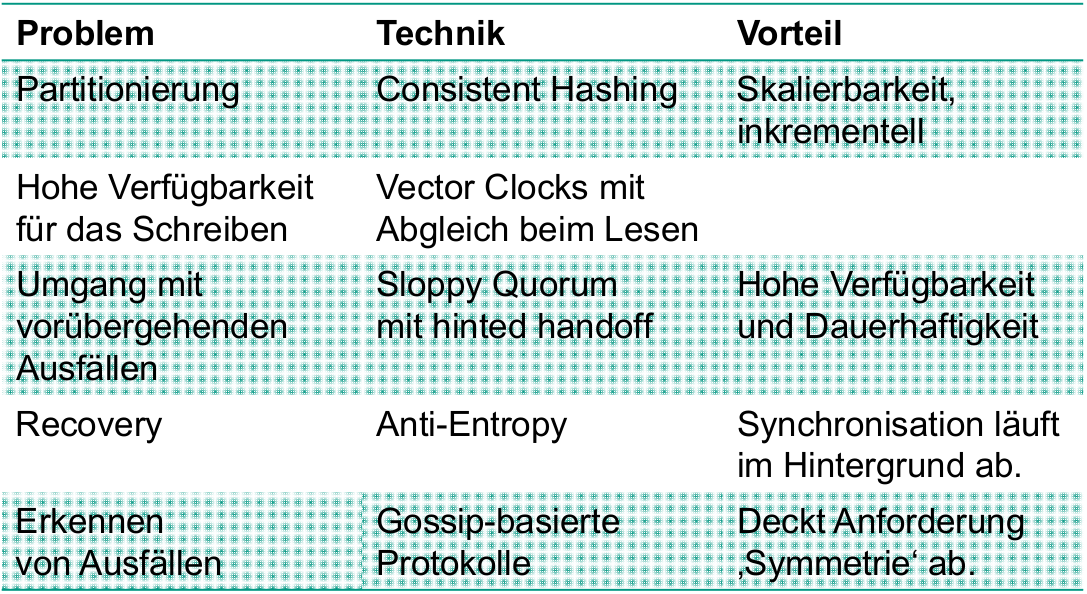
\includegraphics[width=0.33\textwidth]{UebersichtDynamo}\end{figure}

\paragraph{Dynamo --- Vector Clocks}
\begin{itemize}
	\item Ziel: eventual consistency
	\item Liste von (Knoten, Zähler)-Paaren (eine Liste pro Version) \( \leadsto \) Erfassung der Zusammenhönge zwischen Versionen
	\item Quorum-basierte Techniken \( \leadsto \) Inkonsistenzen vermeiden
	\item Vector-Clock-basierte Techniken \( \leadsto \) Inkonsistenzen erkennen und auflösen
	\item Unterschiedliche Knoten können Schreiboperationen absetzen \\* \( \leadsto \) Eine Liste von (Knote, Zähler)-Paaren pro Version
	\item Version 1 ist Vorgänger von Version 2, wenn jeder Zähler in Liste von V1 einen kleineren Wert hat als in der von V2
	\item Update (put) muss festlegen, welche Version aktualisiert werden soll
	\item Get gibt i.A. mehrere Versionen zurück
	\item Kombination mit \emph{Sloppy Quorum}: \( Q_R+Q_W < N \)
\end{itemize}



\paragraph{Datenbanktechnologie auf Dynamo}
\begin{itemize}
	\item Dynamo kein DBS im klassischen Sinn: Niedrigere Schnittstelle für Anwendungsentwicklung
	\item Aber: Bessere nichtfunktionale Eigenschaften
	\item Im Folgenden: Ansätze für DBS 'On Top of' Dynamo
\end{itemize}

\paragraph{Scale Independence}
\begin{itemize}
	\item Anfrage ist \emph{scale-independent}
		\\*
		\( \leadsto \) Laufzeitverhalten unabhängig von DB-Größe
	\item Anfragenklassifikation nach Aufwand: \\*
		- Klasse I (konstant):
			\\*
			z.B. Schlüssel-Zugriff, \lstinline[language=sql]{LIMIT}-beschränkt, Paginierung\\*
			Join auf Fremdschlüssel \\*
		- Klasse II (beschränkt):
			\\*
			Explizite Begrenzung liegt vor
			\\*
			Als Kardinalität im erweiterten DB-Schema darstellbar \\*
		- Klasse III (linear / sublinear):
			\\*
			z.B. Ausgabe aller Kunden/Produkte
		\item Klasse IV (superlinear):
			\\*
			z.B. Clustering-Algo, der Self-Join der zugrundeliegenden Relation ausführt
	\item \( \leadsto \) \emph{PIQL} (\emph{performance insightful query language}) - Scale Independent durch Erweiterungen und Beschränkungen der Anfragesprache
\end{itemize}

\paragraph{Physische Optimierung}
\begin{itemize}
	\item Zwei Arten von physischen Operatoren: \\*
		1. \emph{remote operator}: Zugriffe auf key-value store und elementare Verarbeitungsschritte \\*
		2. Client-seitige Operatoren für Query-Logik
	\item Remote Operator: Muss explizite Beschränkung der Größe (und damit der Ausführungsdauer) des Zwischenergebnisses enthalten (i.A. \lstinline{dataStop}-Operator; Fehlermeldung und Nichtausführung wenn dies nicht der Fall ist)
	\item Remote-Operatoren: \\*
		- \emph{IndexScan}: Prädikat muss zusammenhängendem Ausschnitt des indexierten Wertebereichs entsprechen,\\*
		``Sort'' muss Sortierreihenfolge des Index sein \\*
		- \emph{IndexForeignKeyJoin}: Beschränkung durch Fremdschlüsseleigenschaft \( \leadsto \) kein logischer Stop-Operator, linker Teilausdruck enthält Fremdschlüssel \\*
		- \emph{SortedIndexJoin}: Bei Sortierung des Inputs nach Join Key lässt sich aus limit hint-Begrenzuung der Anzahl an Datenobjekten pro Schlüssel ableiten
\end{itemize}

\paragraph{SLO Compliance-Vorhersage}
\begin{itemize}
	\item SLO = \emph{serivce-level objectives}
	\item Größenbeschränkung Zwischenergebnisse noch keine Garantie für insgesamt beschränkten Aufwand
	\item Wenn anliegende Last sehr groß kann IndexScan-Ausführung beliebig lange dauern
	\item Histogramm-Lookup über Zufallsverteilung (Tupelgröße, Anzahl erwarteter Tupel)
\end{itemize}

\begin{fragen}
	\item Was für Möglichkeiten kennen Sie, den Join zu implementieren? Weche Komplexität haben sie?
	\item Welche Möglichkeiten kennen Sie, den Aufwand, den eine Anfrage verursacht, zu reduzieren/begrenzen?
\end{fragen}
  \section{Anwendungsentwicklung}
\label{sec:anwendungeentwicklung}

\paragraph{Client-Server-Architektur}
\begin{figure}[H]\centering\label{ClientServer}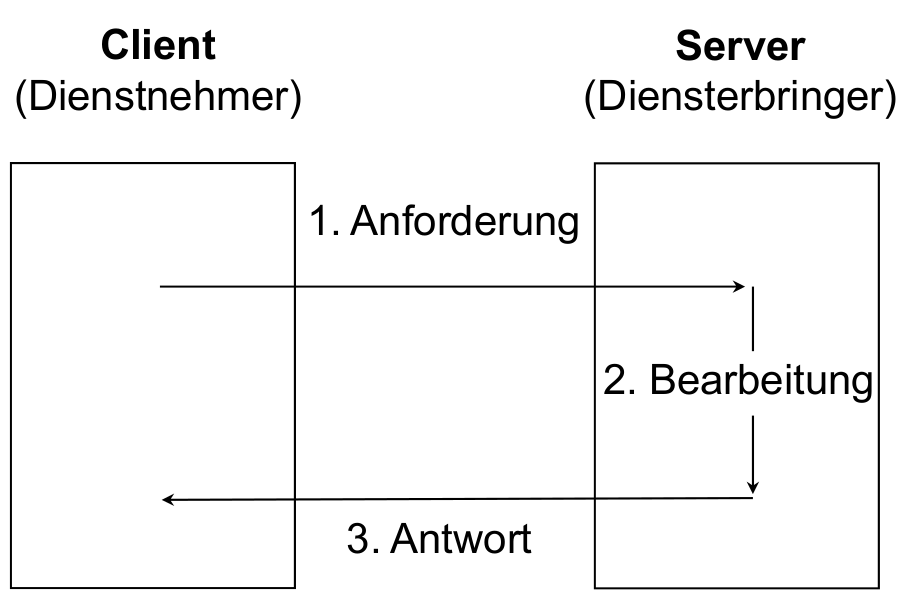
\includegraphics[width=0.25\textwidth]{ClientServer}\end{figure}
\begin{items}
	\item Erfordert \\*
		- Kenntnis über angebotene Dienste \\*
		- Protokoll zur Regelung der Interaktion
\end{items}

\paragraph{Zwei Schichten-Architektur}
\begin{figure}[H]\centering\label{ZweiSchichtenArchitektur}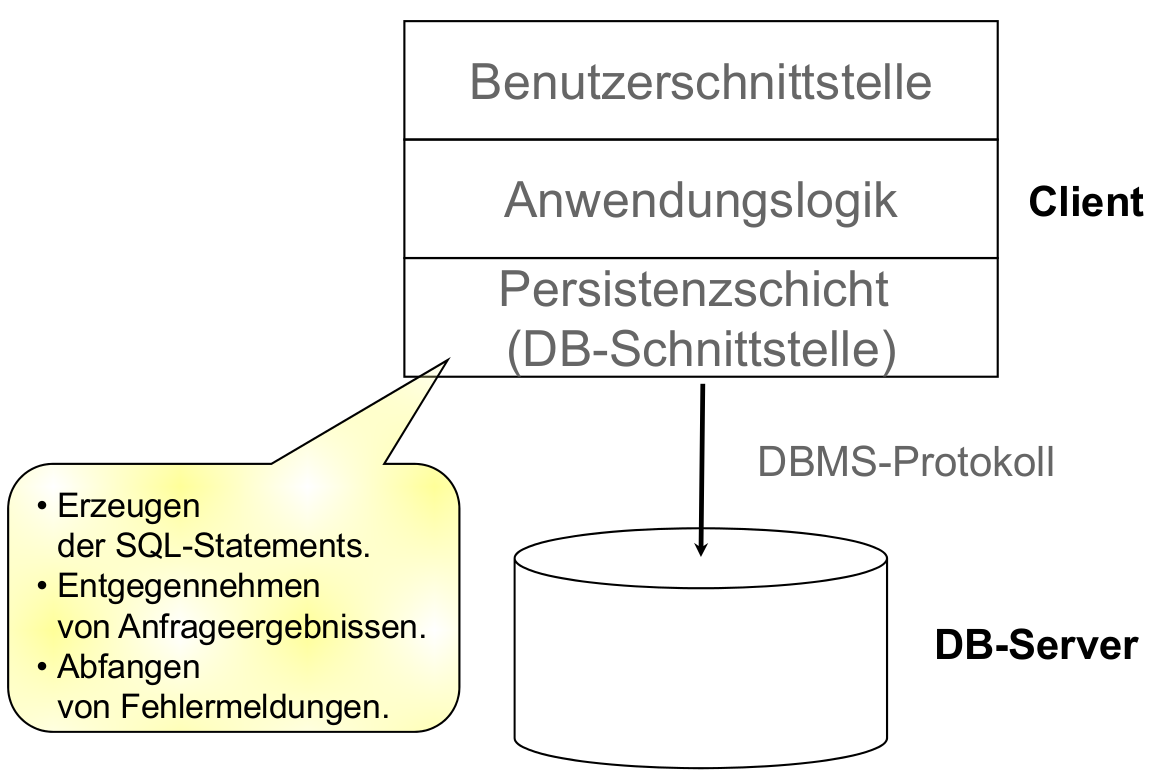
\includegraphics[width=0.33\textwidth]{ZweiSchichtenArchitektur}\end{figure}

\paragraph{Drei Schichten-Architektur}
\begin{figure}[H]\centering\label{DreiSchichtenArchitektur}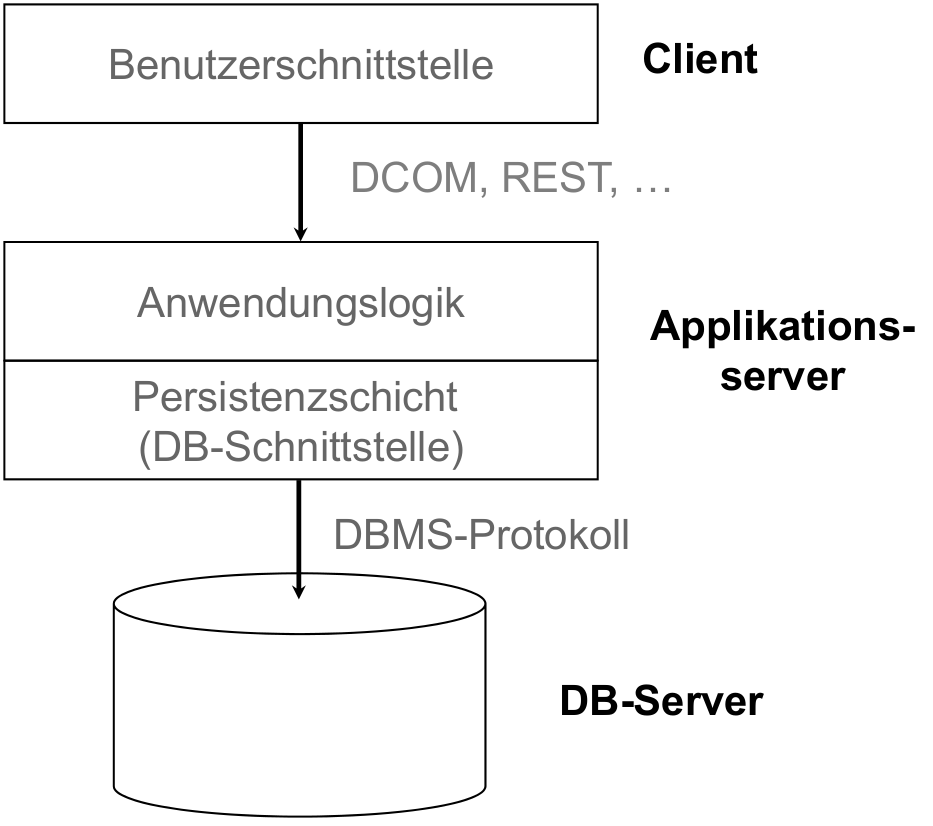
\includegraphics[width=0.33\textwidth]{DreiSchichtenArchitektur}\end{figure}

\paragraph{Anwendungslogik}
\begin{items}
	\item \textbf{Anwendungslogik}: Algorithmen, die anwendungsspezifisches Wissen beinhalten
	\item Personal-DB entählt Mitarbeiter-Daten
		\\*
		\( \leadsto \) Anwendung: schlägt Teamleiter für konkrete Projekte vor
		\\*
		\( \leadsto \) Bedeutsamkeit der Fähigkeiten usw. Anwendungsteil
\end{items}

\paragraph{Cursor-Konzept}
\begin{items}
	\item Cursor \( \equiv \) Iterator
	\item Programmiersprachen: einzelne Datenobjekte als zugrundeliegende Struktur
\end{items}



\paragraph{Programmiersprachenanbindung}
\begin{figure}[H]\centering\label{Programmiersprachenanbindung}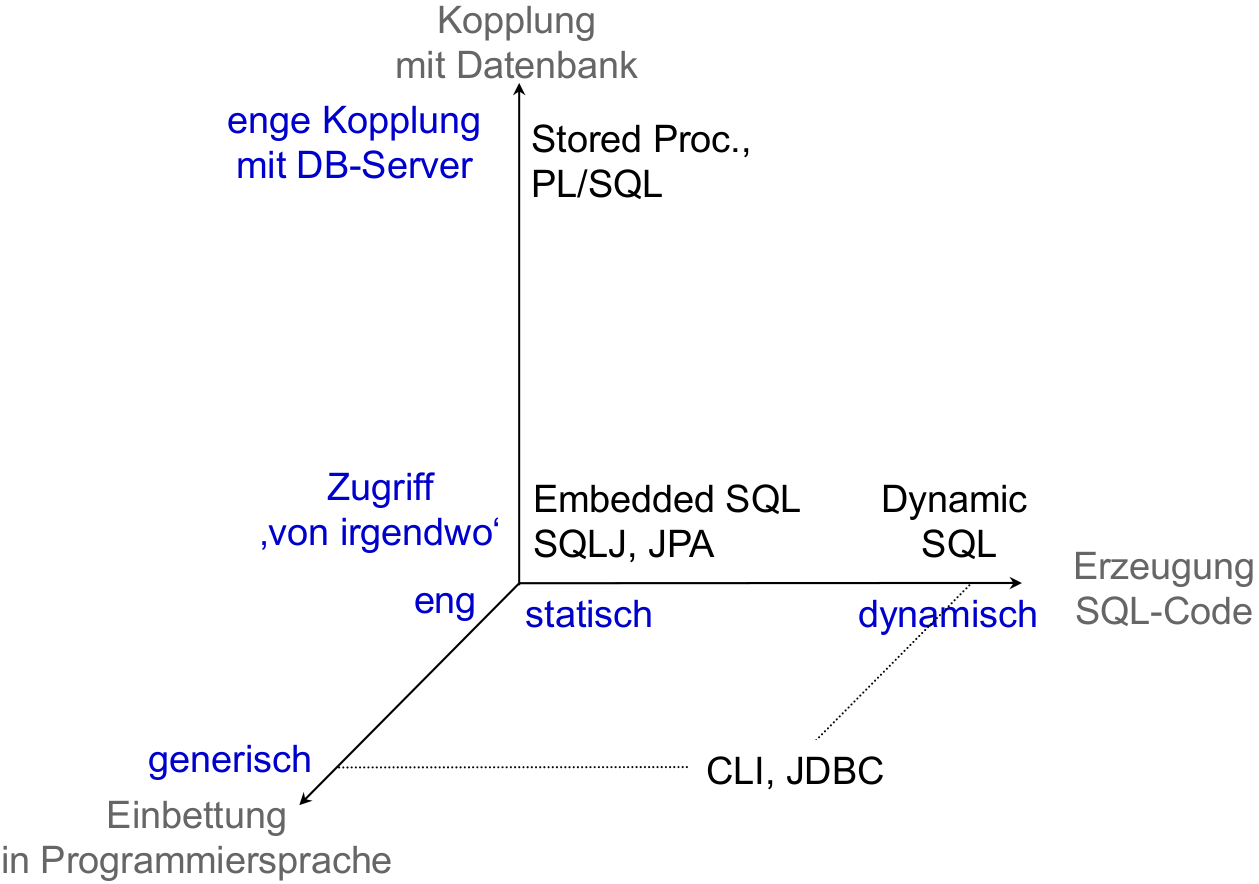
\includegraphics[width=0.33\textwidth]{Programmiersprachenanbindung}\end{figure}

\paragraph{Prepared Statements}
\begin{items}
	\item Reduzieren Ausführungszeit, da bereits vorab kompiliert
	\item
		\begin{lstlisting}[language=java,showstringspaces=false]
PreparedStatement updateSales = 
  con.prepareStatement('UPDATE COFFEES 
  SET SALES = ? WHERE COF_NAME LIKE ?');
		\end{lstlisting}
	\item \lstinline[language=java]{upcdateSales.setInt(1,75);}
\end{items}

\paragraph{Gespeicherte Prozeduren}
\begin{items}
	\item In DB-Server verwaltete und ausgeführte Software-Module in Form von Prozeduren/Funktionen
	\item Aufruf aus Anwendungen/Anfragen heraus
	\item \( \leadsto \) Weniger Kontextwechsel in Anwendung
\end{items}

\paragraph{Variablen und Typen}
\begin{items}
	\item \lstinline[language=sql]{DECLARE preis NUMBER;}
	\item Stellt sicher, dass Attributtyp in DB identisch zu Typ in Programm ist
\end{items}

\paragraph{Kontrollfluss}
\begin{items}
	\item
	\begin{lstlisting}[language=sql]
DECLARE
  a NUMBER;
  b NUMBER;
BEGIN
  SELECT e,f INTO a,b
  FROM T1 WHERE e>1;
  IF b=1 THEN
    INSERT INTO T1 VALUES(b,a);
  ELSE
    INSERT INTO T1 VALUES(b+10,a+10);
  END IF;
END;
.
run;
	\end{lstlisting}
\end{items}

\paragraph{Performance Anti-Patterns}
\begin{items}
	\item \textbf{Excessive Dynamic Allocation}:
		\\*
		Häufige unnötige Objekterstellung/-zerstörung derselben Klasse
	\item \textbf{The Stifle}:
		\\*
		Unpassende DB-Schnittstellennutzung
	\item \textbf{Circuitous Treasure Hunt}:
		\\*
		Abfrage von Relation A, damit Relation B abfragen,\dots
	\item \textbf{Sisyphus DB Retrieval}:
		\\*
		Riesige Datenmenge abfragen, obwohl nur wenige Einträge nötig
	\item \textbf{Spaghetti Query}:
		\\*
		Mehrere Informationsbedürfnisse in einer Anfrage
	\item \textbf{Insufficient Caching}:
		\\*
		Zu wenig Caching
	\item \textbf{Wrong Caching Strategy}:
		\\*
		Falsche Objekte werden in Cache abgelegt
\end{items}

\begin{fragen}
	\item Erläutern Sie die Dimensionen des Raums der Möglichkeiten des Zugriffs auf Datenbanken aus Anwendungen heraus.
	\item Erläutern Sie die Begriffe \\*
		- Anwendungslogik, \\*
		- Cursor, \\*
		- Call-Level Interface, \\*
		- Host-Variablen.
	\item Kann man mit Embedded SQL sicherstellen, dass keine Schema-spezifischen Fehler auftreten? Wenn ja, wie geht es?
	\item Was sind die Vorteile von Stored Procedures? Erläutern Sie das Konzept.
\end{fragen}

\end{document}
